%Inicializacion del documento [tamano de letra, tamano de papel]{clase de documento}
\documentclass[11pt,letterpaper]{article}

%Agrega las referencias a la tabla de contenidos
%\usepackage[nottoc,numbib]{tocbibind}

%Otra fuente (comentar)
%\renewcommand*\rmdefault{ppl}

%Cambiar espaciado entre párrafos
\setlength{\parskip}{3pt}

\usepackage{fancyhdr}
% ajuste de margenes.Se puede omitir, pero a mi no megustan los margenes gigantes que trae por defecto
\usepackage{anysize}
\marginsize{2cm}{2cm}{1cm}{2cm}
% paquetes espa�ol que incluyen � y tildes
\usepackage[utf8]{inputenc}
\usepackage[activeacute,spanish]{babel} 
%paquete para letras con dos rallitas
\usepackage{amssymb,amsmath}
% paquetes imagenes
%\usepackage[rflt]{floatflt}
\usepackage{graphicx}
\usepackage{float}
\usepackage{fancyvrb}
\pagestyle{fancy}
\usepackage{xcolor}
\usepackage[ruled,vlined]{algorithm2e}
%\usepackage{color,soul}
\usepackage{cancel}
\usepackage{wrapfig}%Inclusi�n de gr�ficos al lado de texto
\usepackage{enumerate}
\usepackage{multirow}
\usepackage{subfigure}
\usepackage{pgfplots}
\usepackage{verbatim}
\usepackage{epstopdf}
\usepackage{dsfont}
\usepackage{hyperref}
\definecolor{gray51}{rgb}{0.51,0.51,0.51}
\definecolor{gray31}{rgb}{0.31,0.31,0.31}
\definecolor{gray71}{rgb}{0.71,0.71,0.71}
\usepackage{mathtools}
\DeclareMathOperator*{\argmin}{arg\,min}
\DeclareMathOperator*{\argmax}{arg\,max}

\fvset{frame=single,framesep=1mm,fontfamily=courier,fontsize=\scriptsize,numbers=left,framerule=.3mm,numbersep=1mm,commandchars=\\\{\}}
\definecolor{g}{rgb}{0,0.51,0}
\definecolor{m}{rgb}{1,0,1}
\newcommand{\portada}[9]{
\begin{titlepage}

% Upper part of the page
 

{
\begin{wrapfigure}{l}{.8cm}
\vspace{-.7cm}

\includegraphics[width=4.5cm]{Imagenes/FCFM.jpg}
\end{wrapfigure}
\textsc{\color{red}\hspace{2.7cm}Departamento de Ingeniería Eléctrica}\\
\textsc{\color{gray51}\hspace{3.3cm}Facultad de Ciencias Físicas y Matemáticas}\\
\textsc{\color{gray51}\hspace{3.3cm}Universidad de Chile}\\
\textsc{\color{gray51}\hspace{3.3cm}\small #4}\\
}
% T�tulo
\begin{center}
%~\\[6cm] % original
~\\[4cm]
{\color{gray71}\textsc{#3}}
\HRule~ \\[0.4cm]
{ \Huge \textup \bfseries #1}\\[0.4cm]
{ \Large \textup{#2}}\\[0.2cm]
\HRule ~\\[2.5cm]
\end{center}
\begin{minipage}{.5\textwidth}
~
\end{minipage}
\begin{minipage}{.5\textwidth}
\begin{flushright}
\begin{tabular}{l}
\emph{Profesor:} \\
{\small #5}\\[0.2cm]
\emph{Integrantes:}\\
{\small #6}\\
{\small #7}\\
{\small #8}\\
{\small #9}\\

{\emph Fecha:}\\
{\small \today}
\end{tabular}
\end{flushright}
\end{minipage}
\end{titlepage}
}
\newcommand{\HRule}{\rule{\linewidth}{.4mm}}

\lhead{\small\leftmark}
\rhead{EL5003 - Taller de proyecto}
\cfoot{\thepage}
%\numberwithin{figure}{section} %Hace que la primera figura de cada sección X sea X.1
%\numberwithin{table}{section}
\begin{document}
\SetKwBlock{Initp}{Inicialización de parámetros}{}
\SetKwBlock{Initv}{Inicialización de variables}{}
\renewcommand{\tablename}{Tabla}
%\renewcommand{\thealgorithmcf}{\roman{algorithm}}
\renewcommand{\algorithmcfname}{Algoritmo}%
\renewcommand{\thetable}{\arabic{section}.\arabic{table}}
\renewcommand{\thefigure}{\arabic{section}.\arabic{figure}}
\renewcommand{\theequation}{\arabic{section}.\arabic{equation}}
\renewcommand{\listtablename}{Índice de tablas}
\renewcommand{\listfigurename}{Índice de figuras}

\portada{Taller de Proyecto}{Iluminación de tendido de fibra oscura\\ \ \\
  \emph{Telecomunicaciones}}{Proyecto: Avance}{EL5003 - Taller de
  Proyecto}{Bunel, Sergio}{Liberman, Sergio}{Peet, Thomas}{Rebolledo,
  Juan}{Sanhueza, Andrés}
%%%%%%%%%%%%%%%%%%%%%%%%%%%%%%%%%%%%%%%%%%%%%%%%%%
\pagenumbering{roman}
\lhead{\small\leftmark}

\newpage
\tableofcontents
\newpage
\lhead{\small Índice de figuras}
\listoffigures
\newpage
%\lhead{\small Índice de tablas}
%\listoftables
%\newpage
\pagenumbering{arabic}
\setcounter{page}{1}
\lhead{\small\leftmark}

\section{Introducci\'on}
\label{sec:intro}

\subsection{Overview del proyecto}
\label{sec:overview}

Durante el semestre de otoño de 2014, en el marco del curso EL5004
(Taller de Proyecto), se encomendó a un grupo de estudiantes de
ingeniería eléctrica de la Universidad de Chile, la planificación,
diseño y evaluación de un proyecto para mejorar la capacidad de
comunicación entre data centers de la empresa Entel S.A. Para ello,
se aprovechó la infraestructura existente de fibra óptica oscura,
que une los data centers en cuestión y que actualmente utilizan los
clientes para acceder a sus planes contratados.

En la primera parte de este informe se discuten los puntos que hacen
razonable y necesario el cambio de paradigma de la red. Para ello, se
exponen las principales diferencias entre una red oscura y una activa,
demostrando las ventajas técnicas, económicas y financieras en favor
de esta última. También se justifica el proyecto exponiendo sus
ventajas cuantitativa y cualitativamente.

Más adelante, se lleva a cabo la caracterización de la red existente.
Este paso exige determinar las variables a manipular durante el 
desarrollo de la solución. A través de la caracterización, se 
evalúan los tipos de implementación tecnológica posibles según los 
criterios introducidos.

Finalmente se presenta el diseño propuesto, la ingeniería de detalle
del mismo y los costos (CAPEX y OPEX) que explican el proyecto. Se
redactaron conclusiones sobre el diseño y planteamientos futuros de
diseño para un mejor despliegue de la red.

En este informe se podrá encontrar el por qué el proyecto es viable y
conviene a Entel el llevarlo a cabo.

\subsection{Objetivos del proyecto}
\label{sec:objetivos}

El objetivo de este proyecto es estudiar tanto la factibilidad técnica
y económica como el diseño final de una red activa de fibra óptica
para la interconexión garantizada de data centers, aprovechando un
tendido de fibra oscura preexistente.

La factibilidad técnica introduce la necesidad de estudiar a fondo la
arquitectura y topología de una red de fibra óptica.

\subsection{Acrónimos}
\label{sec:acronimos}

En el informe se utilizarán las siguientes siglas recurrentemente:
\begin{itemize}
\item \textbf{DC} \emph{Data center} - Centro de datos
\item \textbf{DWDM} \emph{Dense Wavelength Division Multiplexing} - Multiplexación por división de longitudes de onda densas
\item \textbf{EDFA} \emph{Erbium doped fiber amplifier} - Amplificador de fibra dopada en erbio
\item \textbf{FO} Fibra óptica
\item \textbf{GE} Gigabit Ethernet
\item \textbf{MTBF} \emph{Mean Time Between Failures} - Tiempo medio entre fallas
\item \textbf{MTTR} \emph{Mean Time To Repair} - Tiempo medio para reparación
\item \textbf{OADM} \emph{Optical add/drop multiplexor} - Multiplexador óptico de agregación/remoción
\item \textbf{ODF} \emph{Optical Distribution Frame} - Organizador de fibra óptica
\item \textbf{SLA} \emph{Service Level Agreement} - Acuerdo de nivel de servicio
\item \textbf{ROADM} \emph{Reconfigurable optical add/drop multiplexor} - Multiplexador óptico de agregación/remoción
\item \textbf{WSON} \emph{Wavelength Switched Optical Network} - Red óptica conmutada por longitud de onda
\item \textbf{WSS} \emph{Wavelength Selective Switching} - Conmutación de longitud de onda selectiva
\item \textbf{OLA} \emph{Optical Line Amplifier} - Amplificador Óptico de Línea
\end{itemize}
% 1era resumen ejecutivo , overview, objetivos, acronimos
\newpage
\section{Caracterización de la red actual}
\label{sec:caracterizacion}

La red considerada para el comienzo de este proyecto consiste en un
tendido de fibra óptica estándar tipo G.652.D (ver sección
\ref{sec:marcoteorico}). Cada enlace de fibra óptica une un par de
\emph{DC} de forma directa y sin estaciones intermedias mediante
cables de 96 fibras diseñadas para operar en la banda C. Esta red no
posee ningún tipo de multiplexor. En un comienzo, cada fibra tiene
soporte para un solo servicio usando un par de transmisión y recepción
Láser, filtros y amplificadores, donde aplique. Se supone, sin
embargo, que en un comienzo el tendido de fibras es de un punto a otro
entre dos \emph{DC}, sin ningún tipo de equipos instalado.

El tendido inicial es de 399 Km distribuídos en 9 tramos, de los
cuales tres son de distancias mayores a 40 Km. Este tendido tal y como
está no tiene considerado ningún análisis que considere cortes de los
cables, por lo que no existen garantías \emph{SLA} que establezcan
políticas claras de calidad de servicio. Por otro lado, es sabido que
tramos de más de 30 Km. deben ser compensados en atenuación y los
mayores a 40 Km. deben ser compensados en dispersión
cromática. También por esa razón el tendido de fibra oscura no cumple
con el \emph{SLA} establecido en calidad de la señal debido a que no
existen garantías de una correcta recepción de la señal.

Por otro lado, no existen en la red inicial mecanismos íntegros de
recepción, tales cómo equipos de \textit{Optical Distribution Frame
  (ODF)}, equipos Mux/Demux (\textit{ROADM/WSS}) con sus respectivos
\textit{racks} y \textit{shelves}, por lo que la red no resulta
escalable en equipamiento tampoco.

Las aplicaciones de la red actual son limitadas, pero igualmente
tienen algún sentido. Las redes oscuras son una forma precaria pero
rápida de interconectar dos nodos. Si es necesario conectar dos
\emph{DC} a través de un nodo intermedio, un enlace físico debe ser
establecido para que ello ocurra. No hay detalles sobre cómo se
interconectaban los nodos ``discontinuos'', solo lo hay entre nodos
contiguos.

\begin{figure}[h]
\centering
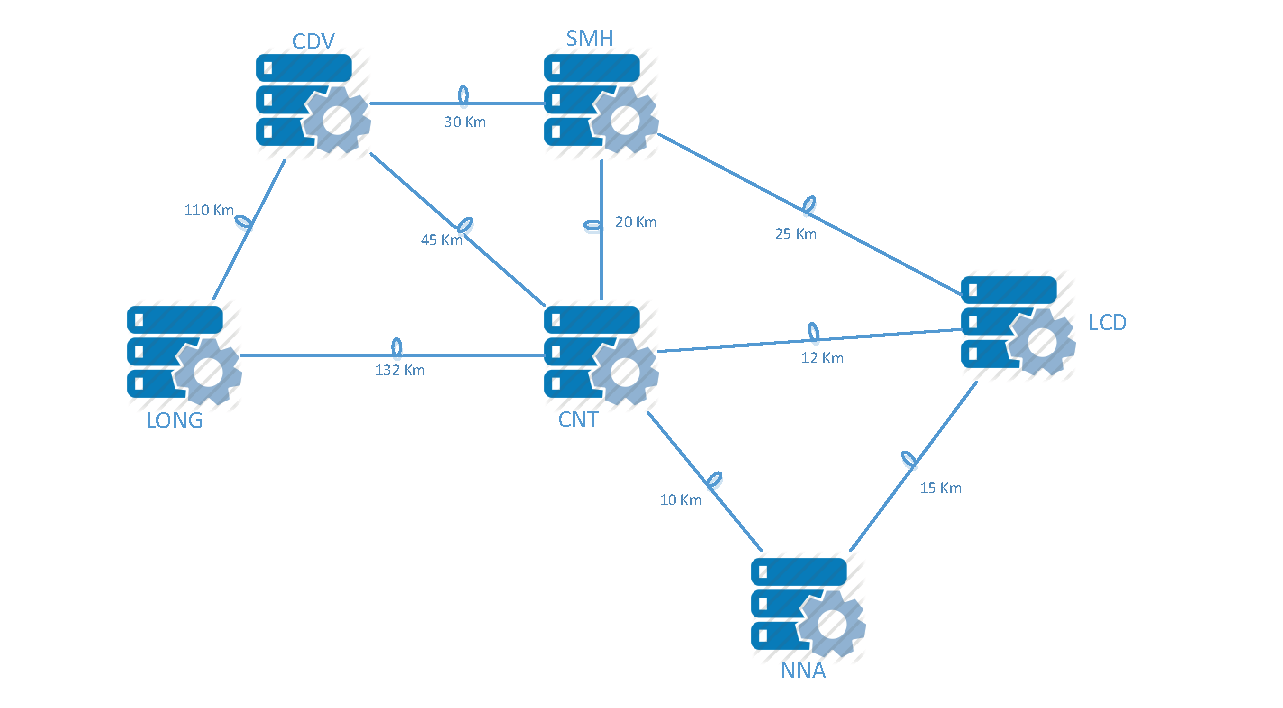
\includegraphics[width=0.8\textwidth]{Imagenes/Diagrama_Fibra_Oscura.eps}
\caption{Diagrama inicial de red oscura preexistente. Este diagrama se
  presenta a los distintos proveedores para poder estimar el
  número necesario de amplificadores, compensadores de dispersión,
  etcétera.}
\label{fig:diagrama_red}
\end{figure}

% Para la caracterización y planificación de la red, se consideran 3
% factores claves en todas sus etapas:

% \begin{itemize}
% \item Delay Introducido
% \item Distancia
% \item Costos Monetarios
% \end{itemize}

% Para la Fibra Oscura:

% Si el delay es considerado, se puede incluir cómo un costo adicional
% de distancia (sabiendo la relación entre cantidad de saltos y
% distancia), de tal forma que la minimización ocurra en torno a una
% sola variable.

% Una vez resueltos los costos en una sola variable (Saltos y
% Distancia), se procederá a minimizar la función costo usando el
% conocido algoritmo de Dijkstra.

% Adicionalmente a este procedimiento, para el caso de posibles cortes
% simultáneos, ha de hacerse un estudio probabilístico, dependiendo de
% que tan probable es que se corte una fibra según un umbral ``$\mu$'' se
% dispondrá de una o más rutas alternativas para esta.

% Visualización del estado actual del servicio que entrega la red. Fibra oscura botada, falta de equipo.
\newpage

\section{Marco Te\'orico}
\label{sec:marcoteorico}

\subsection{Tecnolog\'ias en redes fot\'onicas}
\label{sec:redfotonica}

\subsubsection{Fibra de tipo G.652.D}

Como ya se ha dicho en secciones previas, la fibra oscura de la que se
dispone en el tendido preexistente es del tipo G.652.D. Sus
características ópticas se muestran en la tabla \ref{fig:tablafibra}.

\begin{figure}[H]
  \centering
  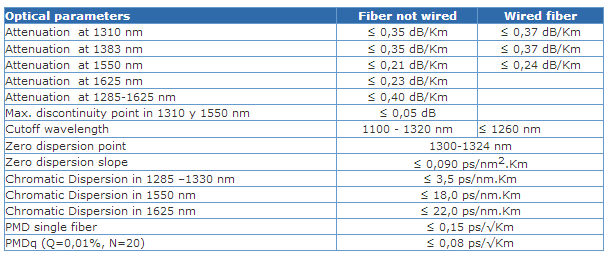
\includegraphics[scale=1]{Imagenes/Fibra.png}
  \caption{Carácteristicas ópticas fibra G.D652.D \cite{datasheetfibra}}
  \label{fig:tablafibra}
\end{figure}
  
Es sabido el hecho de que las fibras ópticas son muy susceptibles a
los factores medioambientales, siendo dentro de los más sensibles la
penetración de agua, vibración, cambios de temperatura y ataques
biológicos (e.g. roedores). También afectan para tendidos
aéreos las cargas de viento y hielos.

\subsubsection{DWDM}
\label{sec:dwdm}

Las redes de fibra óptica modernas utilizan una tecnología de
transporte de alta capacidad llamada \emph{Dense Wavelength Division
Multiplexing} (\emph{DWDM} o en español \emph{multiplexación densa de 
longitud de onda}). Esta tecnología permite introducir varias señales 
con distinta frecuencia a una misma fibra óptica mono modo, permitiendo 
transmisiones con mayores anchos de banda.\cite{dwdm1}\cite{dwdm2}

\emph{DWDM} opera en la capa de red, por lo que es independiente de
los protocolos de transporte y enlace. La multiplexación ocurre sobre
la banda C, es decir, a partir de la longitud de onda 1529,16 nm y
hasta 1560,61 nm ($\lambda$ central = 1510 nm). En frecuencias, esto
corresponde al rango entre 192100 GHz y 196000 GHz (frecuencia
central: 1931000 GHz).

A medida que aumentan los avances tecnológicos, los módulos que
trabajan con esta técnica de multiplexación incorporan mayor capacidad
al condensar cada vez más los canales en el espacio de frecuencia,
aumentando la cantidad de señales en una sola fibra. En la actualidad,
la mayor parte de las empresas de telecomunicaciones realiza diseños
que consideran espaciamientos de 100 o 50 GHz, lo que se traduce en
enlaces de 40 ú 80 canales (o $\lambda$'s) respectivamente. No
obstante, la ciencia ya experimenta con canales espaciados por 25 e
incluso 12,5 GHz solamente, pudiendo llegarse a incorporar en el
futuro hasta 320 $\lambda$ en una sola fibra. 

En la jerga de telecomunicaciones ópticas, a los distintos $\lambda$
se les llama también ``colores'', por la similitud de conceptos en la
óptica de comunicaciones y la óptica tradicional.

\begin{figure}[H]
  \centering
  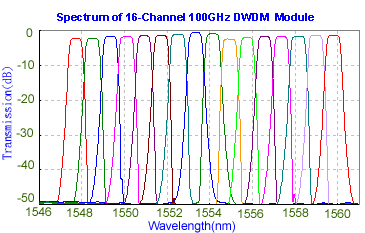
\includegraphics[scale=1]{Imagenes/DWDM_channels.png}
  \caption{Representación en el espacio frecuencial de distintas
    señales multiplexadas sobre la banda C utilizando DWDM.\cite{bandasdwdm} Se
    observan 16 canales de los 40 disponibles con un espaciamiento de
    100 GHz.}
  \label{fig:dwdmchannels}
\end{figure}

\subsubsection{OADM}
\label{sec:oadm}

Los dispositivos que se encargan de agregar o quitar $\lambda$'s de la
fibra con el fin de controlar el enlace por donde se encausan las
señales a enviar se llaman \emph{OADM}, siglas de ``optical add-drop
multiplexer''.

Existen dos tipos de \emph{OADM}. El más primitivo es el \emph{FOADM},
donde la F significa ``fixed'', es decir, fijo o estático. Este tipo
de direccionamiento no es reconfigurable, es decir, el diseño de la
red debe incluir los dispositivos que harán el encausamiento en los
nodos requeridos, sin permitir cambio dinámico de canales en la
fibra. En \emph{FOADM}, los filtros o LASER debían ser fijados en los
nodos, acorde a las necesidades de la red al momento de su diseño. En
el caso de requerir un cambio en la red se debían cambiar y reconectar
jumpers, debiendo detener el funcionamiento de la red por el tiempo
que este proceso demorase. Además, la granularidad o precisión del
encausamiento era de por lo menos $2\lambda$, lo cual introducía
despilfarro de recursos en la red, disminuyendo el ancho de banda de
la red a al menos la mitad.

Debido a este inconveniente, se creó y rápidamente se reemplazó el
\emph{FOADM} por el \emph{ROADM}, con la R de
``reconfigurable''. Estos dispositivos son reprogramables remotamente,
e incluso la conmutación puede cambiar de acuerdo a la demanda de
forma dinámica y automática. Su granularidad es de tan solo
$1\lambda$, convirtiéndose en la única opción realmente factible y
adecuada para diseñar redes escalables en el tiempo.

Los dispositivos \emph{ROADM} han evolucionado desde su primera
incorporación al mercado\cite{roadmevolves}. En un principio, los 
\emph{ROADM} debían realizar demultiplexación y multiplexación de
todos los canales para poder manejar eficientemente las señales,
además de varios otros inconvenientes. Esto elevaba notablemente el 
costo de la red pues para minimizar las pérdidas en los nodos se 
debían utilizar transpondedores de mejor calidad.

Los \emph{ROADM} de segunda generación mejoraban en algo los problemas
en la calidad de señal y permitían un switching de mayor calidad para
longitudes de onda individuales utilizando ``Wave Blocking'' (\emph{WB})
o bloqueo de onda. El \emph{WB} solucionaba varios de los problemas que
tenían los dispositivos \emph{ROADM} de primera generación, pero aún no
eran lo suficientemente robustos, pequeños y útiles para ser utilizados
a todo nivel, siendo las redes con \emph{ROADM} de segunda generación 
usualmente utilizadas sólo a nivel de redes metropolitanas.

La tercera generación de \emph{ROADM} hace uso de unos módulos
llamados \emph{WSS} (\emph{wavelength selective switch}). Esta
especificación introduce la capacidad de hacer redes totalmente
flexibles, de forma dinámica y sin necesidad de tener a técnicos
capacitados en la configuración de redes con \emph{OADM} fijos. 
Adicionalmente a la mejora tecnológica, los precios de los
dispositivos disminuyeron puesto al gran aumento de la oferta de
soluciones \emph{DWDM} integrados con \emph{ROADM}.

Otra de las bondades que trajo la introducción de los \emph{WSS} fue
haber incorporado la funcionalidad para interconectar redes de
distintas topologías (redes en anillo y redes en malla, por
ejemplo).

Las funcionalidades actuales de un \emph{ROADM} con \emph{WSS} son las
siguientes:
\begin{itemize}
\item \textbf{Add}: añade una señal externa a la red existente DWDM
\item \textbf{Drop}: extrae una señal de la red en el nodo donde se ejecuta la
  acción
\item \textbf{Switch}: se configura un nodo para unir dos redes y poder
  encausar el $\lambda$ a un nodo de otra red
\item \textbf{Pass-through}: se configura un nodo para no alterar a un
  $\lambda$
\end{itemize}

\subsubsection{Compensadores de atenuación}
\label{sec:amplificadores}

Se utilizan amplificadores ópticos para evitar la excesiva atenuación
de señal en el nodo de destino. Los amplificadores se clasifican según
su ubicación en el enlace\cite{G663}.

El \textbf{booster amplifier} es un dispositivo que se inserta 
directamente después del transmisor óptico. Es especialmente útil en
aplicaciones donde los \emph{OLA} o amplificadores intermedios no se
pueden y/o quieren insertar por algún motivo de diseño (e.g. redes 
submarinas). El ruido que insertan es despreciable, pero una mayor 
potencia a su salida repercute en distorsiones no lineales de la fibra
óptica. En ocasiones, los transmisores incluyen uno de estos
amplificadores.

El \textbf{preamplificador} va en el receptor y sirve para mejorar la
lectura de la señal por parte del dispositivo óptico de destino. En 
ocasiones, éste puede ir en el mismo módulo del receptor.

Los \textbf{optical line amplifiers} o amplificadores de línea sirven para
aumentar la potencia de forma de poder abarcar distancias de hasta miles
de kilómetros. Demasiados \emph{OLA} pueden aumentar el efecto de la
dispersión cromática no lineal y, sobre todo, aumentar los niveles de
ruido a niveles inmanejables, deteriorando demasiado el servicio de
distribución.

Todos los amplificadores pueden diseñarse de forma que el ruido que
inserten sea lo más acotado posible. Ello se logra introduciendo
filtros pasa banda adecuados a los diseños. Habiendo buenos
estándares, los filtros pueden ser diseñados de forma óptima para
casos generales.

La tecnología actual más típica de amplificadores aprovecha un
fenómeno físico del erbio ($Er_{68}$) que, al ser utilizado como
material dopante de fibra óptica y en presencia de una bomba de
fotones, amplifica la señal completa e introduce un ruido altamente
predecible y lineal. Estos amplificadores se llaman por sus siglas en
inglés \emph{EDFA} (\emph{Erbium Doped Fiber Amplifier}).

En este diseño solamente se usaron amplificadores booster y
preamplificadores, ya que las distancias de los enlaces no eran
suficientemente largas para introducir amplificadores de línea.

\subsubsection{Compensadores de dispersión}
\label{sec:dispersion}

La dispersión cromática es un efecto indeseable en las redes fotónicas
multicanal como lo es, en particular, la tecnología \emph{DWDM}. La
disepersión provoca que una señal se ensanche en el dominio de la
frecuencia (o lo que es lo mismo, que se afine en el dominio del
tiempo), haciendo que sea más probable la interferencia entre
$\lambda$'s de distintos canales. Afortunadamente, este fenómeno está
ampliamente estudiado y se sabe con bastante precisión cómo reducir su
efecto a un mínimo, al menos en su componente lineal, predominante en
señales con intensidades ``pequeñas''.

Existen dos enfoques para combatir la dispersión cromática lineal. Uno
es usando \emph{DSP} (procesamiento digital de señales) y el otro
usando dispositivos \emph{DCM} (dispersion compensation module). El
más relevante de estos enfoques y el más utilizado es el \emph{DCM}.

Todas las fibras ópticas tienen un coeficiente de dispersión cromática
que las caracteriza. El coeficiente depende de $\lambda$ y sus
unidades son $\frac{ps}{nm \times Km}$. Los \emph{DCM} son
dispositivos que se especifican en el mercado de acuerdo a su
distancia de fibra a compensar. Tienen un coeficiente de dispersión
negativo que contrarresta el efecto de la fibra en cuanto a la
dispersión que ella intrínsecamente provoca en la señal.

Además del efecto lineal de la dispersión, existen efectos no lineales
que se suman y que son muchísimo más complicados de compensar. Estos
son la \emph{SPM} (self phase modulation) y \emph{XPM} (cross phase
modulation). Estos efectos se producen ya que el campo eléctrico se
modula a sí mismo a medida que avanza en la fibra (cuando éste es lo
suficientemente grande, los efectos de \emph{SPM} y \emph{XPM} toman
mayor importancia).

\subsection{Dispositivos presentes en una red fotónica}
\label{sec:dispositivos}

A continuación se presenta un resumen de los elementos esenciales para
una red óptica basada en DWDM. Estos componentes llevan a la práctica
las tecnologías nombradas en la sección anterior.

\begin{itemize}
\item \textbf{Transpondedor}: ermite transformar una señal de
  algún protocolo de transporte típico (e.g. señales eléctricas) en
  ondas transmitibles por \emph{FO} (señales ópticas) y vice versa.
\item \textbf{Multiplexor/Demultiplexor}: los multiplexores permiten
  combinar señales con distinta longitud de onda provenientes de 
  entradas independientes y enviarlas por una salida común. Los
  demultiplexores hacen lo inverso; seleccionan una de las longitudes
  de onda de la entrada única y la transmiten a una salida individual.
\item \textbf{Amplificadores Ópticos}: mencionados en la sección 
  anterior, restauran la señal a un nivel apropiado para su uso en
  los componentes de la red (e.g. transporte por fibra, conmutación, 
  multiplexación y demultiplexación).
\item \textbf{Canal Óptico de Servicio}: este canal se ubica en una
  frecuencia fuera de la banda C estándar (1510 nm, nominalmente
  hablando). Sirve para transportar señales de alarma entre los
  componentes internos de la red (e.g. conmutadores).
\end{itemize}
% Estado de la tecnología, elementos de la red que se deben considerar.
\newpage
\section{Justificaci\'on del Proyecto}\label{sec:justificacion}

A medida que crece el requerimiento de ancho de banda de los usuarios
en internet, las empresas proveedoras del servicio deben utilizar más
y mejores tecnologías extensibles y flexibles que posibiliten este
proceso.

En esta sección se expondrán los detalles de la justificación del
proyecto, es decir, se mostrarán los aspectos cuantitativos y
cualitativos que permitirán convencerse de que el proyecto es
conveniente.

\subsection{Aspectos cuantitativos}
\label{sec:cuantitativos}

Los aspectos que permiten visualizar en forma contable la conveniencia
del proyecto se deben traducir a términos monetarios. El objetivo es
que la empresa pueda ver de forma clara el contraste entre tener una
red de fibra oscura e instalar una red de fibra activa.

Las redes fotónicas ``oscuras'', es decir, sin ningún tipo de
multiplexación o control de las señales al momento de introducirlas en
la fibra, no son adecuadas para montar redes modernas que requieran
grandes anchos de banda. Este es el caso de los enlaces entre 
datacenters, donde el volumen y la importancia de los datos que fluyen
hacia y desde sus nodos deben cumplir con un tiempo de acceso cada vez
más rápido y por un número creciente de usuarios.

En efecto, lo correcto para notar esta diferencia sustancial en este
contexto es considerar la capacidad de un cable de fibra óptica con y
sin multiplexación en frecuencia. Si cada cable de G.652.D tiene 96
fibras en su interior, entonces se pueden conectar un total de 96
servicios por cada cable. Si se considera un canal de ancho 50 GHz y
protocolos Ethernet de 100 GB/s\footnote{Cerca del tope de la
  tecnología existente al momento de elaborar este informe.}, la
capacidad total de una fibra oscura es de 9.6 TB/s. Considerando la
misma configuración de protocolos en una red \emph{DWDM}, el cable
óptico permite el transporte de 80 veces este valor, es decir, cerca
de 768 TB/s, lo que representa una disminución de costo de instalación
de tendido. Para poder alcanzar este ancho de banda de hubiera
necesitado instalar 80 cables de fibra óptica adicionales en cada uno
de los tramos que en total suman 399 Km.

El análisis anterior supone que los tendidos ya se encuentran
empalmados y operando correctamente con cada uno de los servicios
requeridos. Sin embargo, un corte de alguna fibra significaría que
dejarían de operar algunos de los puntos de red, mientras que un corte
en el cable completo significaría el apagado de 80 puntos de red a la
vez, algo que seguramente afectaría el \emph{SLA} y con ello muchos de
los contratos con clientes.

A continuación se muestra una simulación de los costos de romper el
\emph{SLA} con clientes: si se supone que cada puerto operativo tiene
asociado contratos que suman USD \$1.000.000\footnote{Aproximación
  burda; es probable que el orden de magnitud de este valor haya sido
  subestimado.} en ingresos anuales para Entel, la ruptura de un cable
significaría perder alrededor de USD \$30.000.000 de ingresos anuales
en el caso que las empresas involucradas renuncien al caerse el
servicio.

Una fibra activa con sistemas \emph{WSS} y \emph{WSON} para
restablecer las rutas automáticamente significarían un costo inicial 
como el mencionado en la sección \ref{sec:capex}, pero el
costo de romper contratos por \emph{SLA} se ahorraría.

Un análisis cuantitativo menos dramático tiene que ver con el costo de
la mantención de los equipos. Mantener equipos de fibra oscura
requeriría recurrentemente empalmar fibras, tender nuevos cables e
instalar mayor cantidad de \emph{ODFs}. Ello elevaría el costo por mano
de obra pues las obras durarían mucho más. Además, la cantidad de
conexiones que se crearían sería difícil de predecir, haciendo que la 
probabilidad de cometer errores que terminen afectando el \emph{SLA} 
de los clientes aumente considerablemente.

Los puntos cuantitativos negativos de instalar un sistema \emph{DWDM}
que reemplace al tendido de fibra oscura se pueden observar desde el
punto de vista técnico. Equipos más complejos requerirán mano de obra
especializada y aumento en costo de energía. Sin embargo, estos costos
(ver secciones \ref{sec:capex} y \ref{sec:opex}) son marginales con 
respecto al riesgo de afectar al \emph{SLA}.

En síntesis, la comparación es claramente favorable para una red 
iluminada, pues los riesgos que se toman al violar el \emph{SLA} de los
clientes es mayor a cualquier inversión que se pueda realizar. Por ello, 
se recomienda invertir en \emph{iluminar} la red de fibra óptica.

\subsection{Aspectos cualitativos}
\label{sec:cualitativos}

Los aspectos argumentables de forma no contable que permiten
establecer la conveniencia del proyecto son los que se muestran en
esta sección.

Como muestra la figura \ref{fig:aumento_bw}, el crecimiento de ancho
de banda a nivel global está en aumento constante. Se espera que este
crecimiento no se detenga nunca, ya que a medida que el ser humano
tiene acceso a más velocidad, sus necesidades y exigencias tecnológicas
aumentan.

\begin{figure}[H]
  \centering
  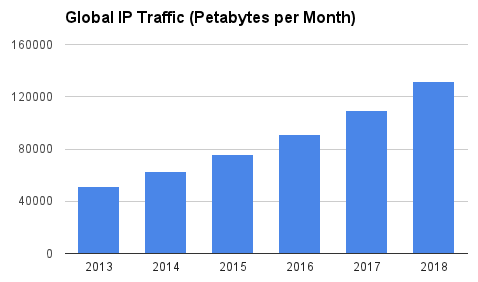
\includegraphics[width=0.75\textwidth]{Imagenes/iptrafficchart.png}
  \caption{Tendencia en el aumento del ancho de banda a nivel mundial
    según un estudio de Cisco de 2014.\cite{ciscoiptraffic}}
  \label{fig:aumento_bw}
\end{figure}

\emph{DWDM} es una tecnología en esencia modular y escalable. Todos
los proveedores de esta tecnología ofrecen actualizaciones en forma de
módulos para poder reemplazar los equipos obsoletos con versiones
nuevas o bien para expandir y mejorar el soporte de las tecnologías
tradicionales a más tendidos.

La incursión de los \emph{ROADM} hacia un sistema programable con
variedad de filtros integrados y con manejo de eventos, como lo son
los dispositivos \emph{WSS}, ha significado que la flexibilidad de
\emph{DWDM} sea mayor que nunca. Por otro lado, los precios de estos
dispositivos han disminuido de forma considerable en los últimos años,
haciéndose populares y soportados globalmente.

Algunos de los servicios más pintorescos que permiten implementar los
\emph{DC} en el mundo son los que se muestran en la figura
\ref{fig:servicios}.

\begin{figure}[H]
  \centering
  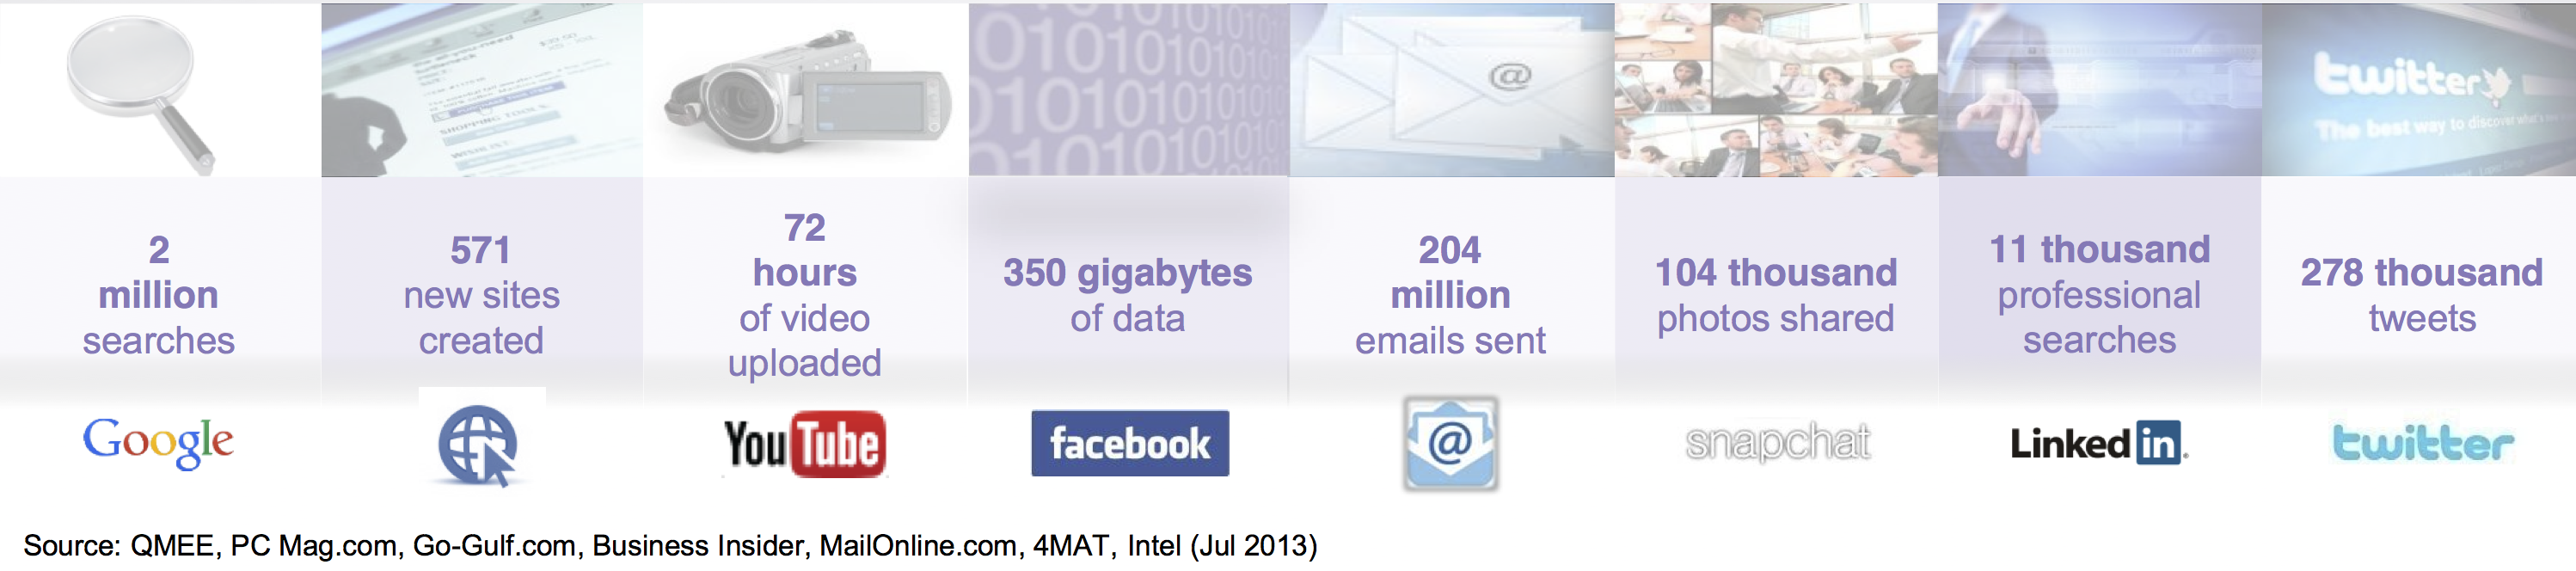
\includegraphics[width=15cm]{Imagenes/servicios.png}
  \caption{Servicios en los que participan \emph{DC} que ocupan una
    muy alta y creciente cantidad de capacidad instalada en las
    redes. Datos de julio de 2013 provenientes de: QMEE, PC Mag.com,
    Go-Gulf.com, Business Insider, MailOnline.com, 4MAT e Intel.}
  \label{fig:servicios}
\end{figure}

Los servicios mostrados en la figura \ref{fig:servicios} son algunos
de los más famosos en la Web a la fecha. Por otro lado, existen 
ambientes de alto tráfico en el ámbito de los observatorios espaciales
y grupos científicos, que deben manejar del orden de petabytes de
información por día. Estos volúmenes de información sólo pueden ser
manejados en la actualidad por \emph{DC}. Sin embargo, el
transporte de estos datos es uno de los cuellos de botella más
críticos del sistema de almacenamiento de información y de las nuevas
tecnologías en el mundo en general.

Este aumento en el flujo de información requiere de redes que se puedan
instalar rápidamente, sin realizar inversiones demasiado grandes y que
tengan la posibilidad de escalar fácilmente en el tiempo. En este
sentido, el argumento nuevamente favorece migrar a \emph{DWDM} en vez
de mantener la fibra oscura. 

En definitiva, los avances, la estandarización y la disminución de
precios que han experimentado este tipo de tecnologías son los
factores más importantes que permiten justificar el proyecto de forma
cualitativa.

% Ver aspectos del estado actual que potencialmente pueden ser mejorados por medio de la ejecución de un proyecto
\newpage
\section{Propuesta}\label{sec:propuesta}

% Propuestas que apuntan a la justificación del proyecto. Iluminar fibra, usar tal cantidad de equipos
% Red optica de data centers
\newpage
\section{Planificaci\'on del Proyecto}\label{sec:planificacion}

La red actual que consta de conexiones físicas de fibra oscura monomodo G.652.D no tiene funcionalidad y no se le esta sacando provecho. Es por esto que se pretende establecer una red inteligente basada en DWDM. La fibra G.652.D posee unas tasas de corte de $0.01$ y $0.05 [\frac{\text{cortes}/\text{año}}{\text{km}}]$ en zona rural y zona metropolitana respectivamente. Dados estos parámetros se desea implementar una red interconectada que garantice cierto estándar de disponibilidad de conectividad entre todos sus puntos.

El diseño de los caminos de la red se realizó utilizando el algoritmo descrito en \ref{sec:algoritmo_conex}. Para entender como funciona el algoritmo hay que definir algunos conceptos preliminares. Existen dos tipos de conexiones: físicas directas y virtuales. Las conexiones físicas corresponden a las fibras oscuras que conectan cada par de datacenter (ver Figura \ref{fig:diagrama_red}. Vale la pena notar que este tipo de conexiones no existe entre todos los datacenter. Distinto es el caso de las conexiones virtuales las cuales pueden ser directas o indirectas. Por ejemplo, una conexión virtual se puede establecer entre los datacenter LONG y CNT a traves de una conexión física directa o entre los datacenter CDV y NNA a través de CNT, estableciendo una conexión entre CDV-CNT y CNT-NNA.

Como cada par de datacenters debe tener una conexión que cumpla con estándares preestablecidos de disponibilidad, se requiere que existan caminos suficientes para que la probabilidad de indisponibilidad (probabilidad de corte acumulado) sea menor al umbral fijado. Los resultados del algoritmo se muestran en la Figura \ref{fig:caminos}.

\begin{figure}[H]
  \centering
  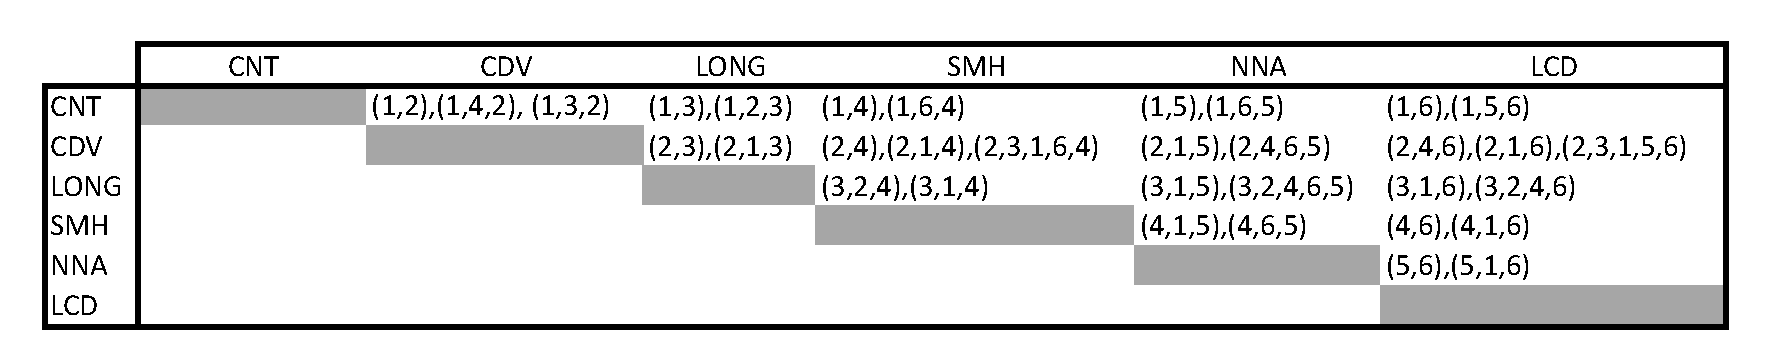
\includegraphics[width=13cm]{Imagenes/caminos}
  \caption[Caminos calculados por algoritmo de disponibilidad]{Caminos que aseguran el estándar de SLA del 0.01\% de indisponibilidad por 2 días. Calculados con algoritmo de la sección \ref{sec:algoritmo_conex}}.
  \label{fig:caminos}
\end{figure}





\begin{itemize}
\item puntos de red a utilizar
\item planos de data centers con distribución de los equipos
\item diagramas de conexión
\item rotulación de fibras, conectores, etc
\item frecuencias
\end{itemize}

% Standby
\newpage
\section{Ingeniería de detalle}\label{sec:ingdetalle}

% Es el conjunto de documentación técnica completa del proyecto que
% permite que la ejecución de éste sea entregada a un tercero y éste
% pueda efectuar la Instalación y Puesta en Marcha con mínimas
% variaciones.

% La Instalación y Puesta en marcha de un proyecto no necesariamente
% debe ser ejecutada por el grupo de trabajo que prepara la Ingeniería
% de Detalle. El ejecutor puede ser otra sección dentro de la misma
% Empresa o una Empresa contratista (Outsourcing). Por este motivo la
% Ingeniería de detalle debe ser completa y muy precisa. No deben quedar
% detalles sin definir.

% Dentro de la Ingeniería de detalle de un proyecto, y dependiendo de la
% naturaleza de éste, se pueden incluir los siguientes elementos:

% Planos de planta de las estaciones, especificando ubicación y
% dimensiones de los racks que alojarán a los equipos nuevos Layout de
% los equipos, esto es, planos frontales de los racks indicando la
% disposición de los equipos.

% Diagramas en bloque de los equipos indicando las interconexiones de
% los diferentes módulos (no se trata de los diagramas de circuitos
% electrónicos de cada tarjeta, información que los fabricantes no
% suelen entregar, sino que de las conexiones externas entre las
% diferentes tarjetas, para conseguir que los equipos trabajen en la
% forma deseada).

% Diagrama de cross-conexiones entre las diferentes interfaces de línea
% y las puertas tributarias de los equipos.  Plan de sincronización de
% la Red Planos de Planta Externa Memorias de cálculo
 
 
% El último elemento requiere de explicaciones adicionales.
 
% Una Memoria de Cálculo, como su nombre indica, es el resultado de los
% análisis y cálculos que efectúa un ingeniero especialista en una
% materia para determinar la forma correcta como debe ejecutarse una
% parte del proyecto para que el sistema funcione correctamente y de
% acuerdo a lo esperado.
 
% La memoria de cálculo puede ser de varios tipos según el
% proyecto. Algunos ejemplos:
 
% Memoria de cálculo de malla de tierra. Arroja como resultado
% especificaciones sobre la geometría de la malla, profundidad y número
% de las barras de cobre que deben enterrarse, valor de resistividad del
% terreno al cual debe llegarse.
 
% Memoria de cálculo de un radio enlace. Incluye un perfil del enlace,
% cálculos de niveles de señal, atenuaciones de las guías de onda y
% filtros, ganancia de las antenas, potencias de salida de los
% transmisores y nivel de recepción. Pero lo más importante es el
% cálculo de predicción de comportamiento del enlace en el peor mes del
% año, esto es \% del tiempo que el enlace estará indisponible (Tasa de
% error peor que 1E-03) y \% del tiempo que el enlace estará degradado
% (Tasa de error peor que 1E-06). Todos los métodos de cálculo y valores
% límites para los porcentajes mencionados están detallados por el ITU.
 
% Memoria de cálculo de enlaces por fibra óptica. Este tema es de
% importancia para el proyecto que les corresponde desarrollar. estos
% cálculos incluyen: balance de potencia; cálculo de razón señal a ruido
% óptica (OSNR) y cálculos de dispersión.
 
% Los resultados de estos cálculos determinan el diseño de la red y por
% lo tanto tiene impacto en el CAPEX y OPEX del proyecto: tipo de
% interfaces ópticas (estándar, de alta potencia, Ultra alta potencia),
% necesidad de usar Amplificadores Ópticos de Línea (OLA) o
% Regeneradores intermedios en un enlace.
 
% El impacto en el CAPEX es claro, si el diseño arroja que es necesario
% incluir una estación regeneradora en medio de un enlace entre
% estaciones ya existentes, el costo del proyecto se eleva notablemente.
 
% Por otra parte, un diseño muy audaz puede significar una reducción del
% margen disponible en el enlace, lo cual ante una degradación menor del
% cable de fibra puede hacer que el enlace se corte o degrade, obligando
% a efectuar mantenimiento con más frecuencia y elevando el OPEX.
 
% Memoria de cálculo de una torre. En un proyecto que incluya enlaces de
% microondas y emplazamiento de radio estaciones nuevas con sus
% receptivas torres, se debe incluir el cálculo de la estructura de la
% torre para asegurar su resistencia al peso de las antenas, al viento,
% etc. Naturalmente este cálculo cae dentro de las responsabilidades de
% un Ingeniero Civil no Eléctrico.

En esta sección se presentará la ingeniería de detalle para el
proyecto de implementación de red óptica utilizando \emph{DWDM} y
\emph{ROADM} con \emph{WSS} basado en un enfoque probabilístico para
diseño de caminos óptimos a partir de valores esperados del
\emph{SLA}.

La ingeniería de detalle expuesta aquí es una recopilación de todos
los documentos técnicos que se requieren para la instalación física de
los equipos y la programación de los \emph{ROADM}. Esta recopilación
se basa en el diseño final seleccionado de entre las propuestas de los
proveedores en la sección \ref{sec:ppfinal}.

\subsection{Diagramas de conexión ROADM}
\label{sec:diagramasroadm}

El detalle de las conexiones de equipos en cada uno de los \emph{DC}
se presenta en las siguientes secciones.

\subsubsection{Conexión ROADM ``Ciudad de los valles''}
\label{sec:drcdv}

\begin{figure}[H]
  \centering
  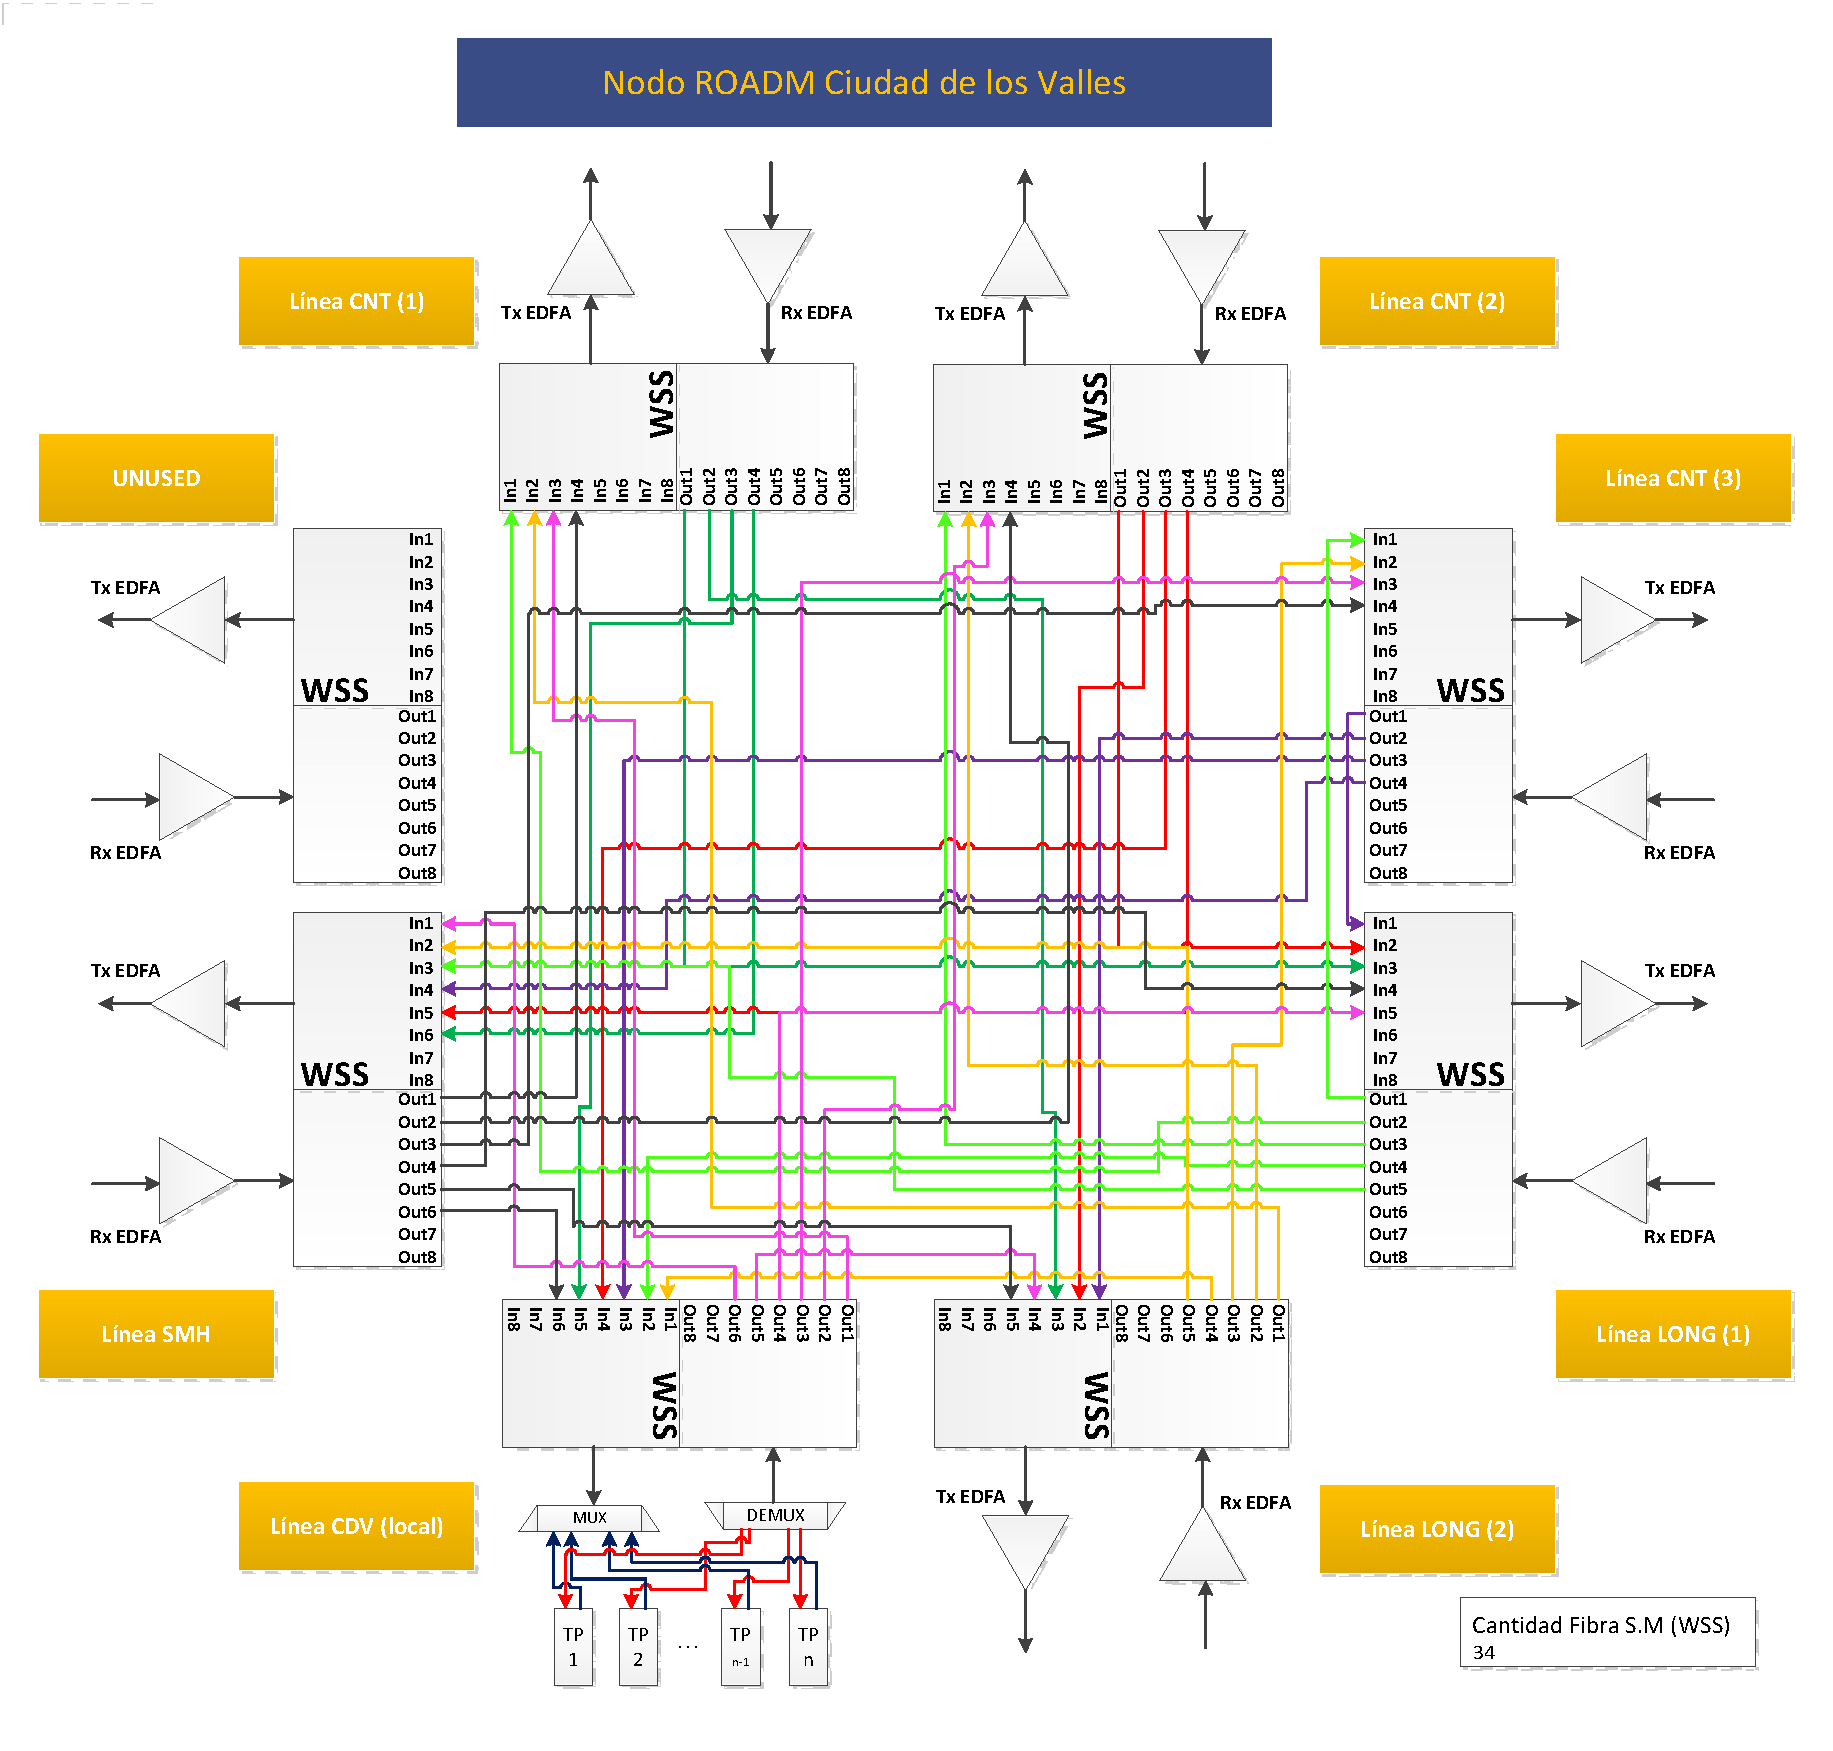
\includegraphics[width=17cm]{Imagenes/CDV.pdf}
  \caption{Diagrama de conexión de equipos para infrastructura ROADM en ``Ciudad de los valles''}
  \label{fig:drcdv}
\end{figure}

\subsubsection{Conexión ROADM ``Central nacional de telecomunicaciones''}
\label{sec:drcnt}

\begin{figure}[H]
  \centering
  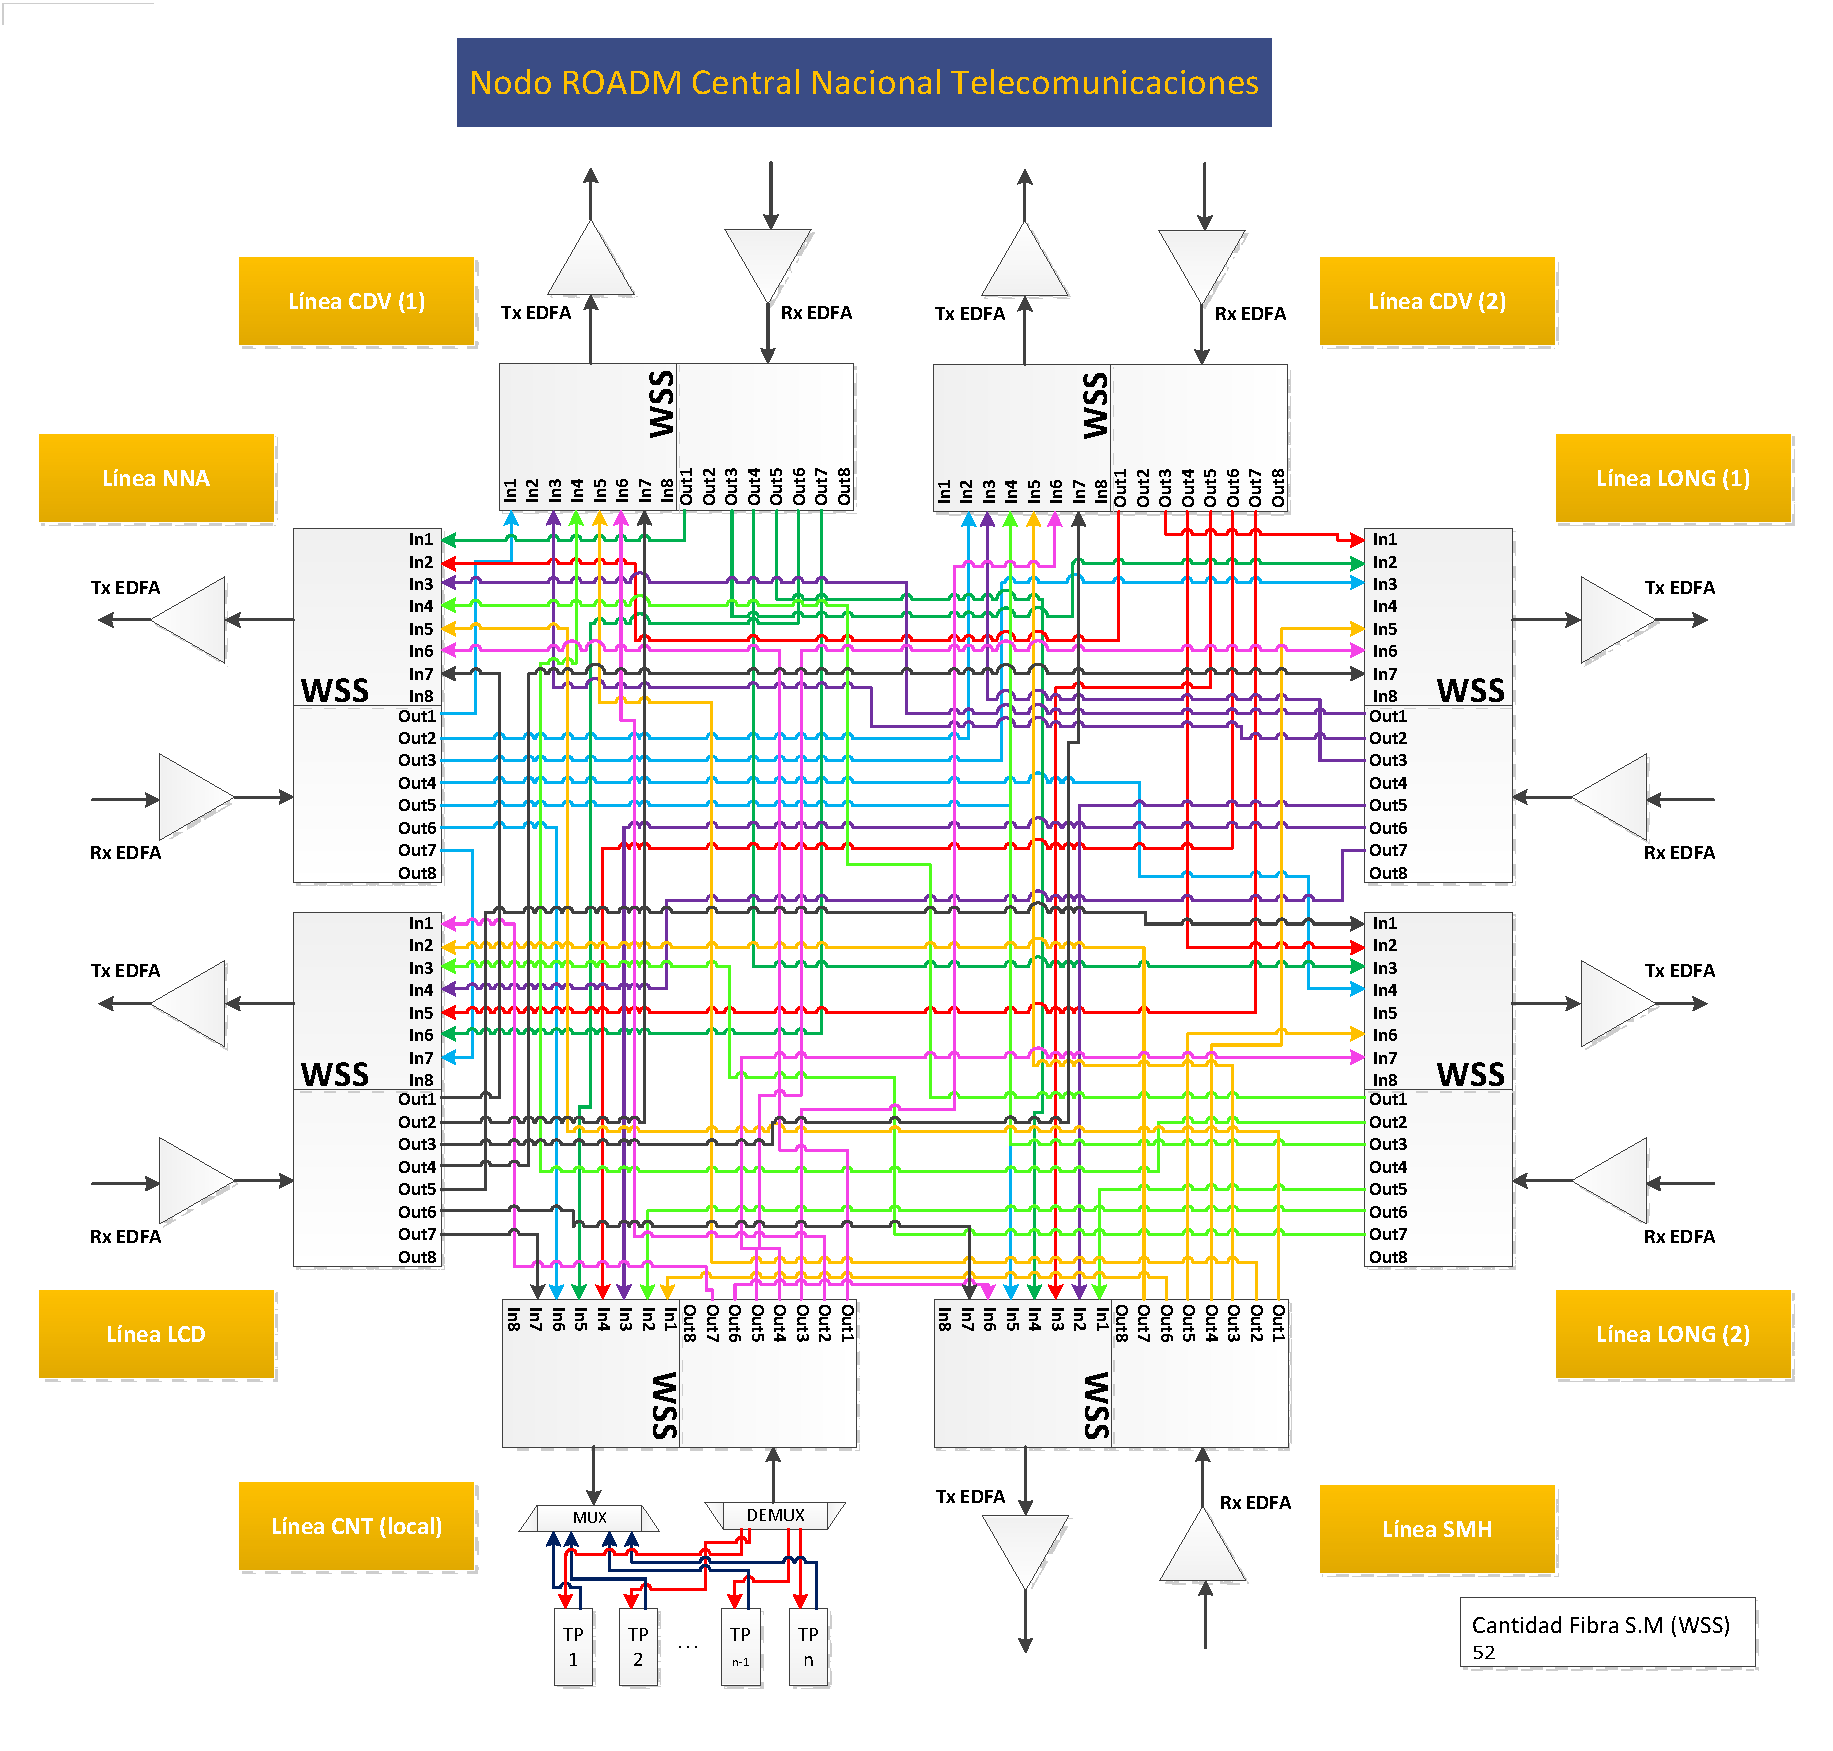
\includegraphics[width=17cm]{Imagenes/CNT.pdf}
  \caption{Diagrama de conexión de equipos para infrastructura ROADM en ``Central nacional de telecomunicaciones''}
  \label{fig:drcnt}
\end{figure}

\subsubsection{Conexión ROADM ``Las Condes''}
\label{sec:drlcd}

\begin{figure}[H]
  \centering
  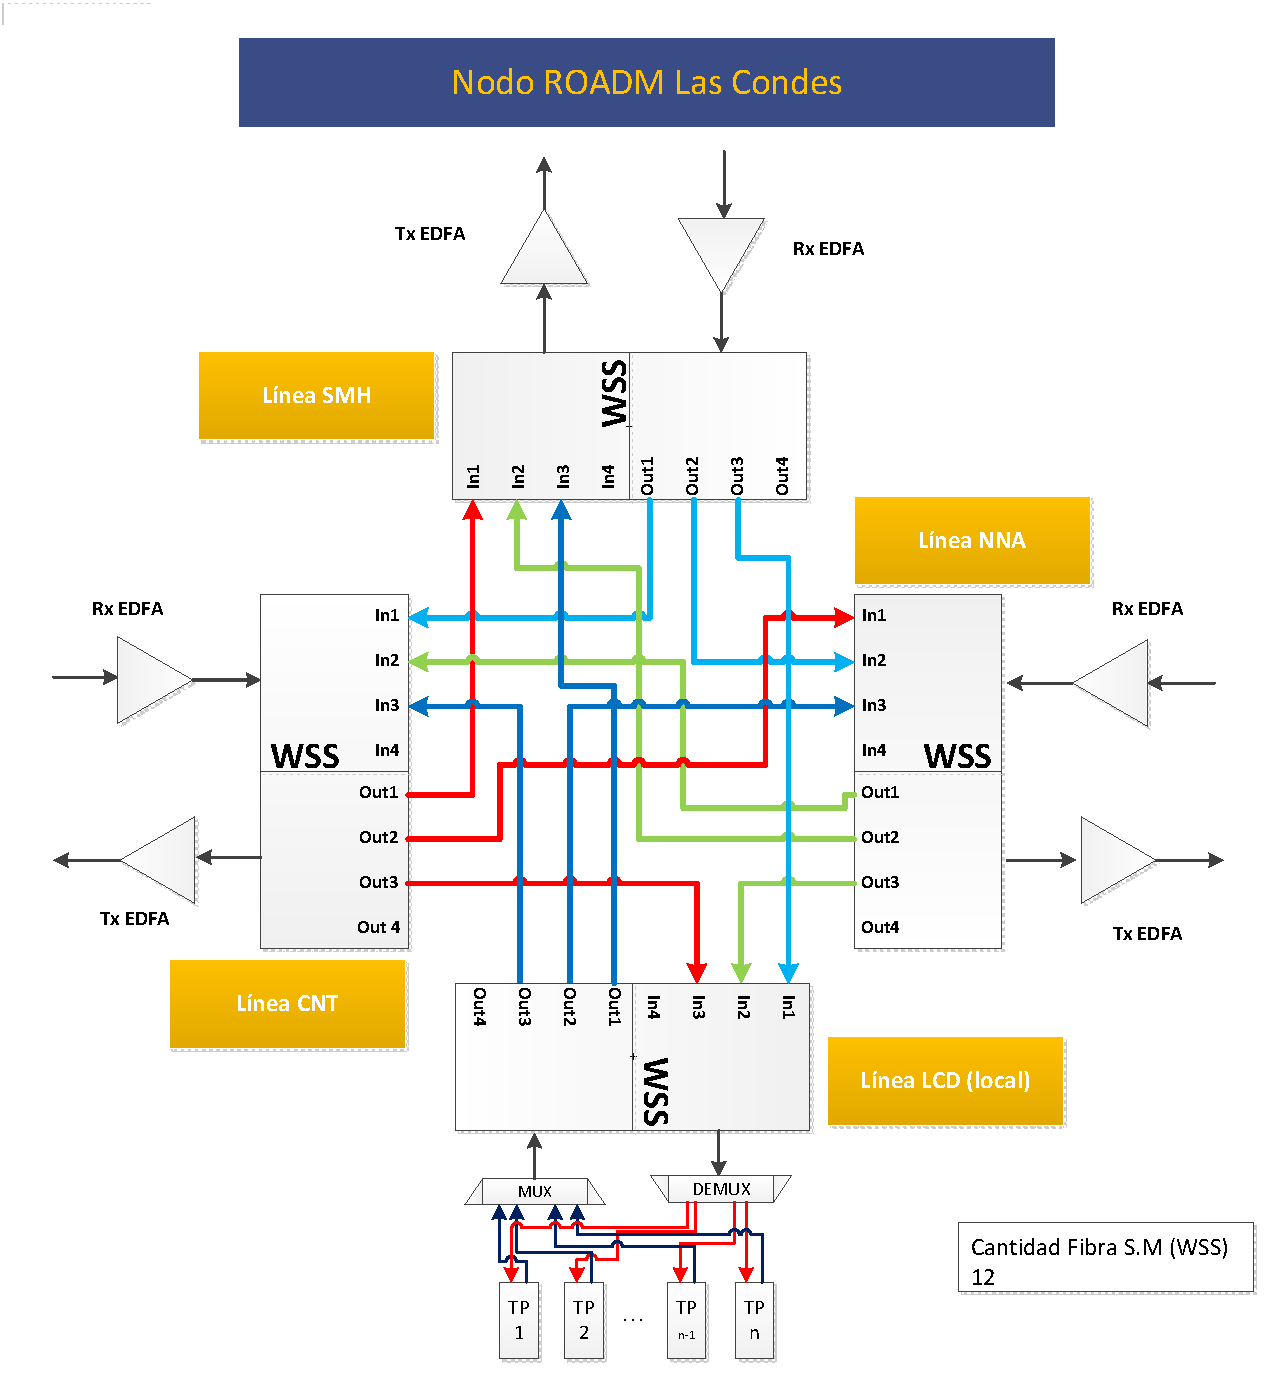
\includegraphics[width=17cm]{Imagenes/LCD.pdf}
  \caption{Diagrama de conexión de equipos para infrastructura ROADM en ``Las Condes''}
  \label{fig:drlcd}
\end{figure}

\subsubsection{Conexión ROADM ``Longovilo''}
\label{sec:drlong}

\begin{figure}[H]
  \centering
  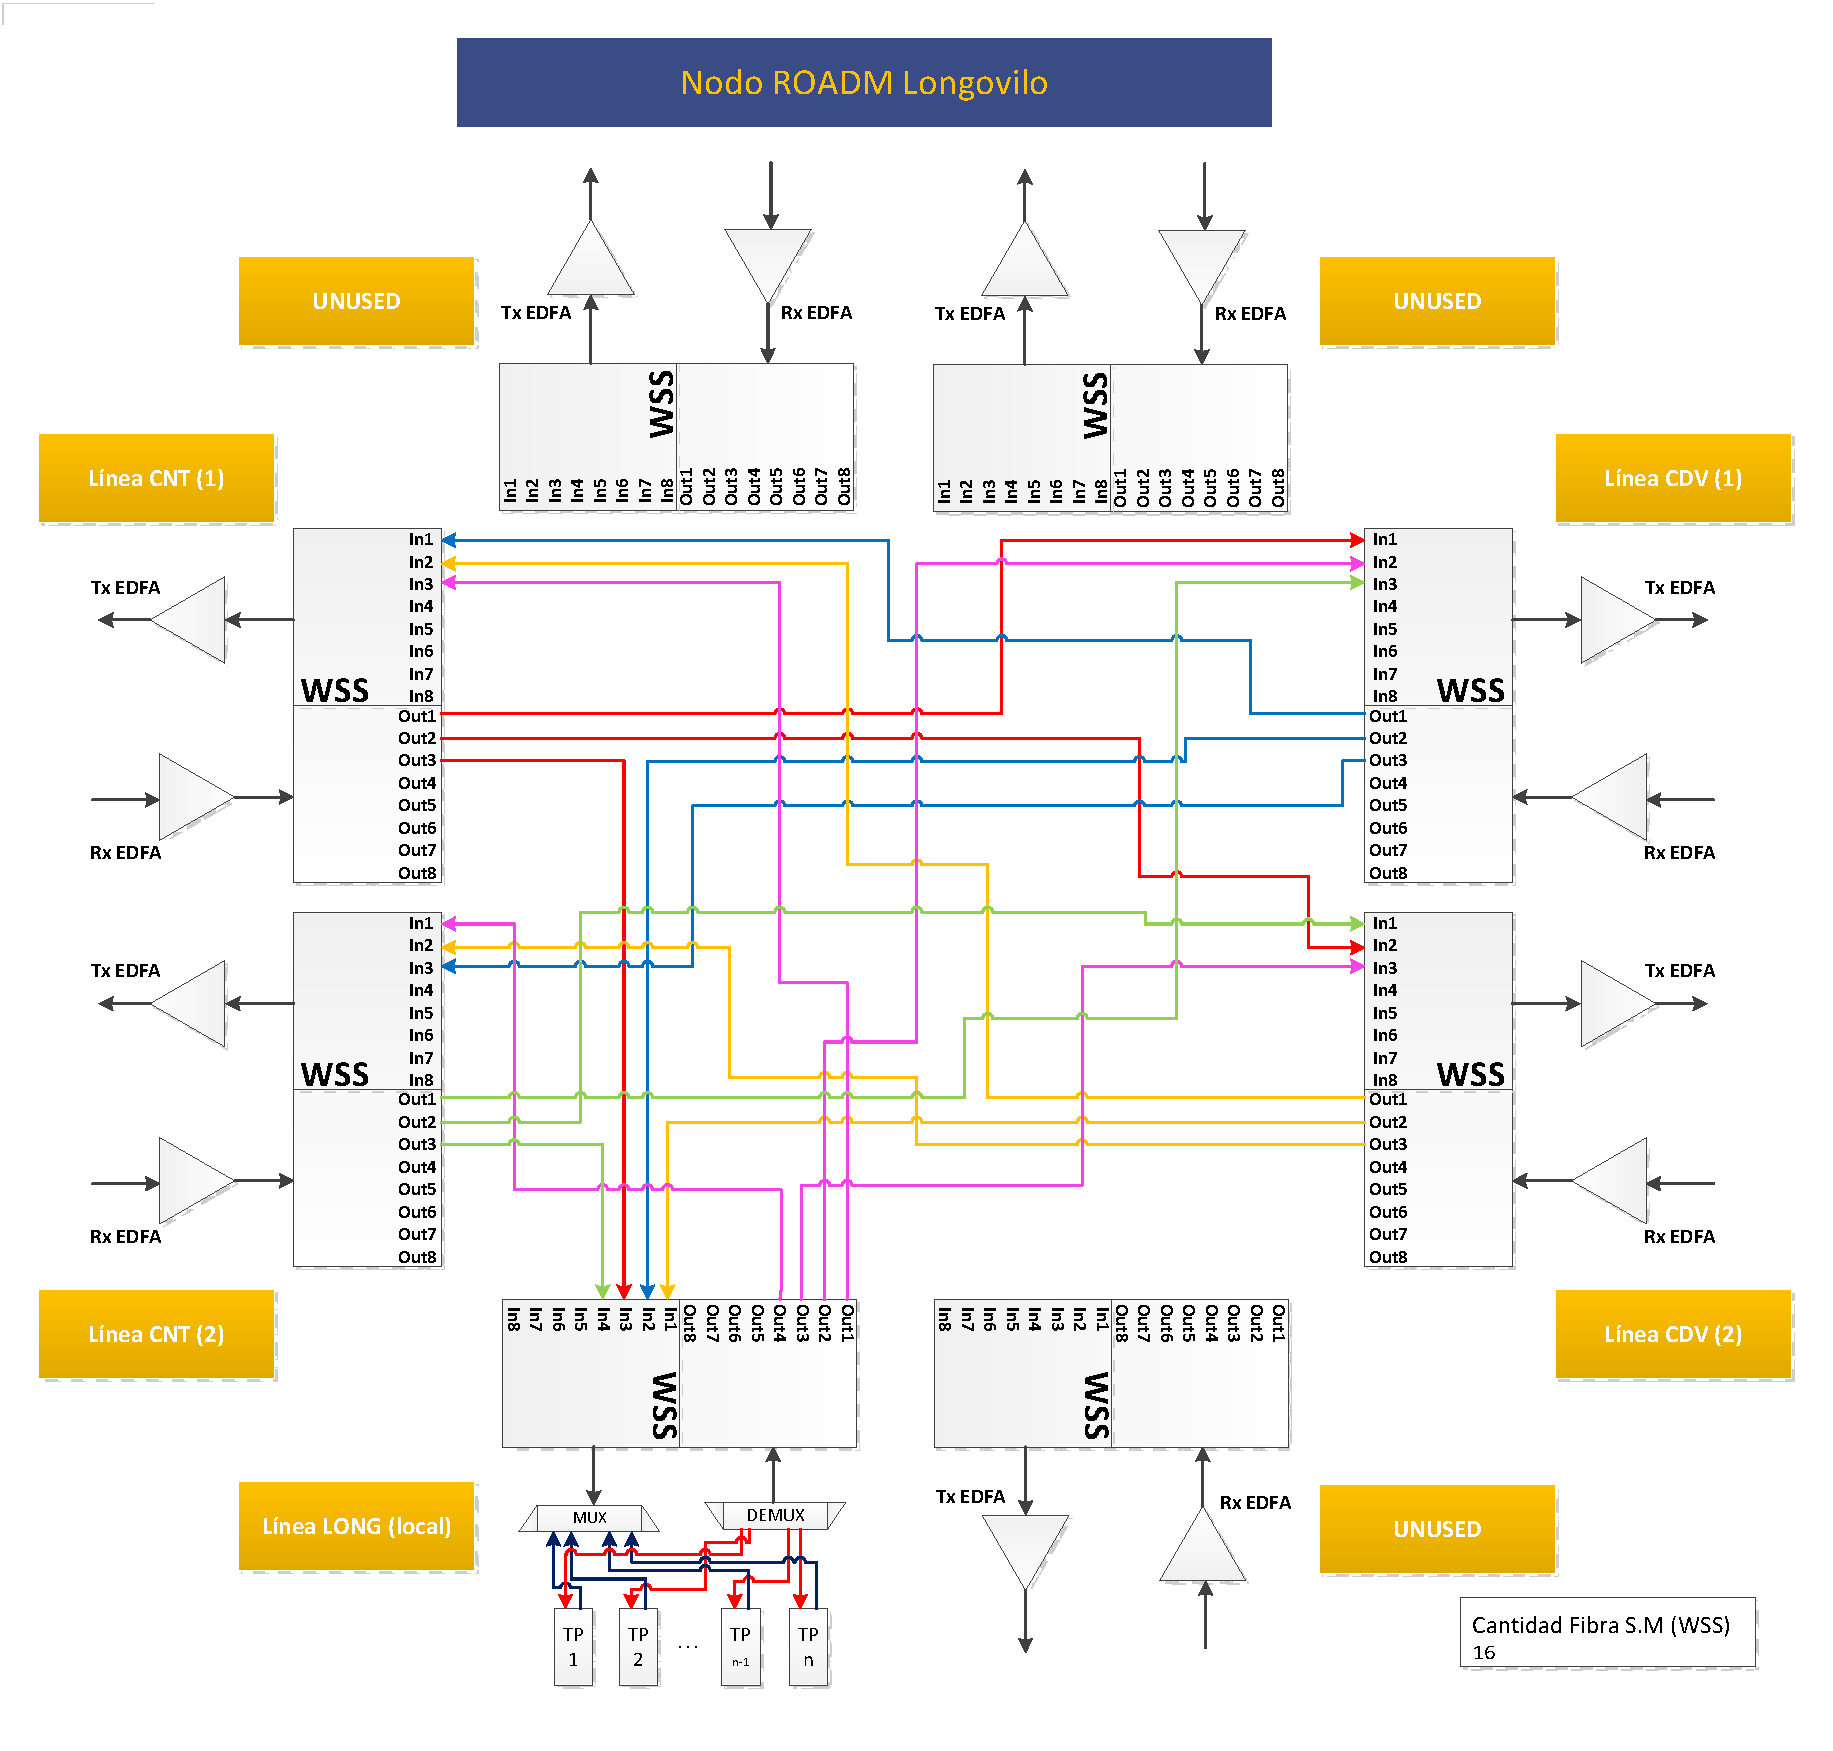
\includegraphics[width=17cm]{Imagenes/LONG.pdf}
  \caption{Diagrama de conexión de equipos para infrastructura ROADM en ``Longovilo''}
  \label{fig:drlong}
\end{figure}

\subsubsection{Conexión ROADM ``Ñuñoa''}
\label{sec:drnna}

\begin{figure}[H]
  \centering
  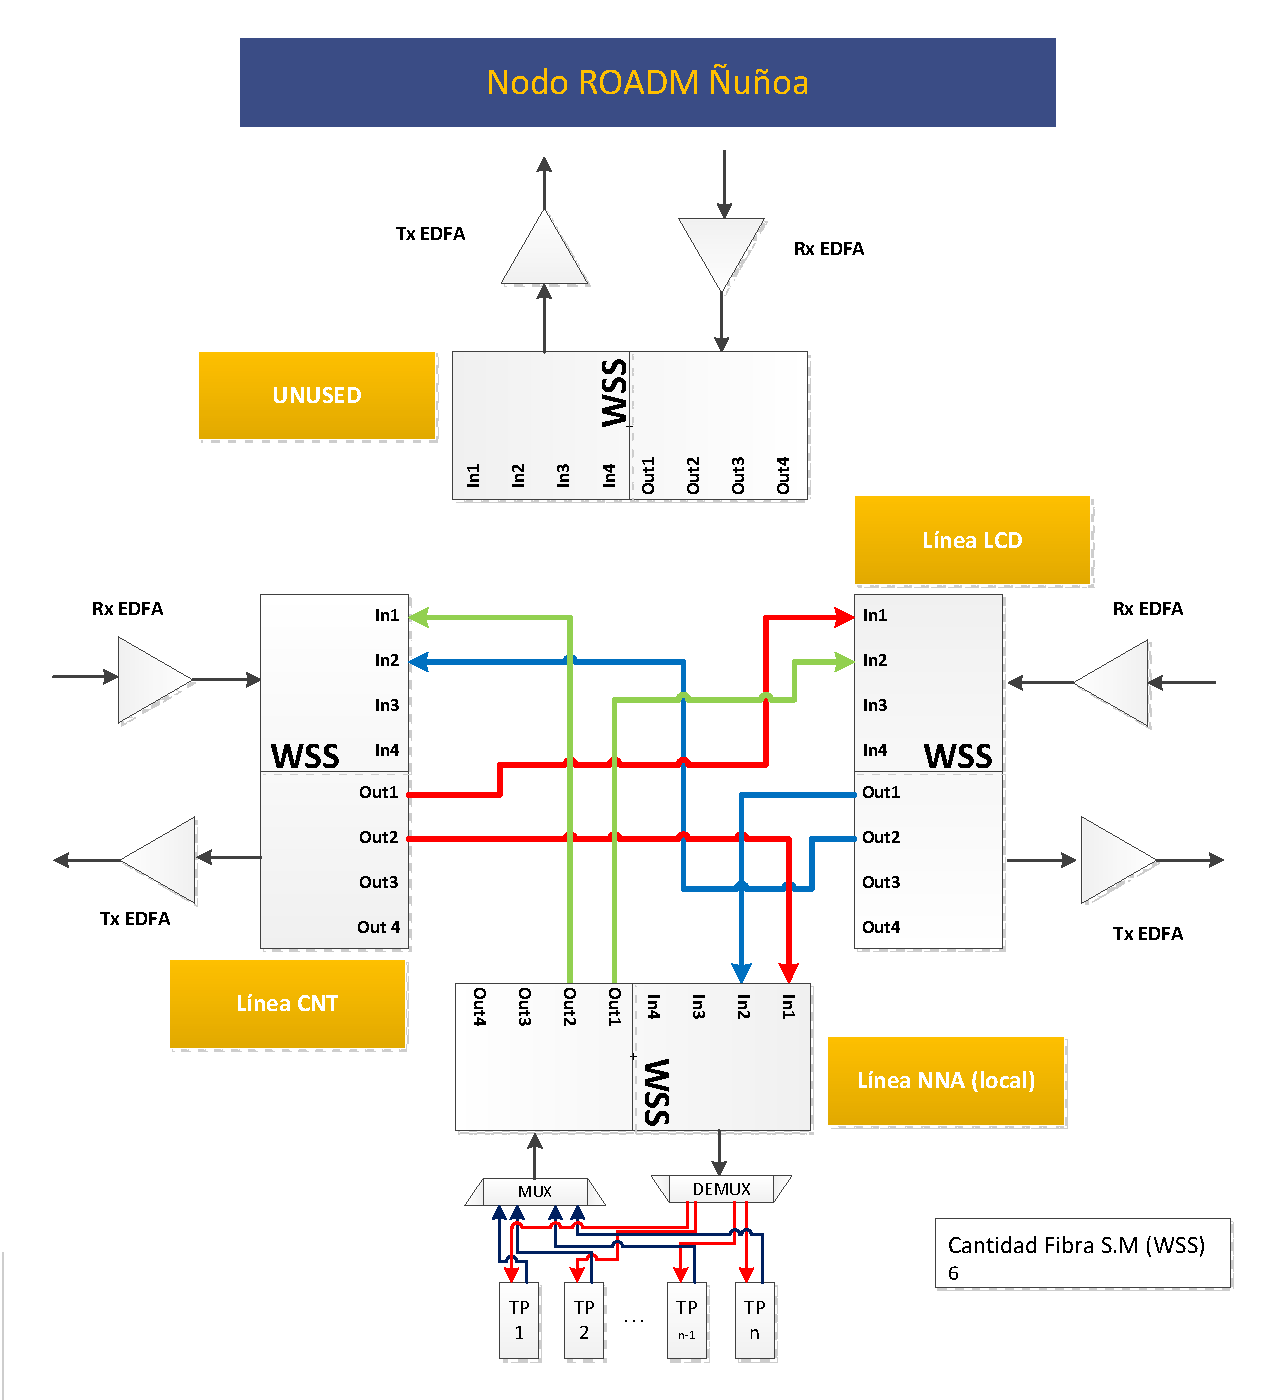
\includegraphics[width=17cm]{Imagenes/NNA.pdf}
  \caption{Diagrama de conexión de equipos para infrastructura ROADM en ``Ñuñoa''}
  \label{fig:drnna}
\end{figure}

\subsubsection{Conexión ROADM ``Santa Marta de Huechuraba''}
\label{sec:drsmh}

\begin{figure}[H]
  \centering
  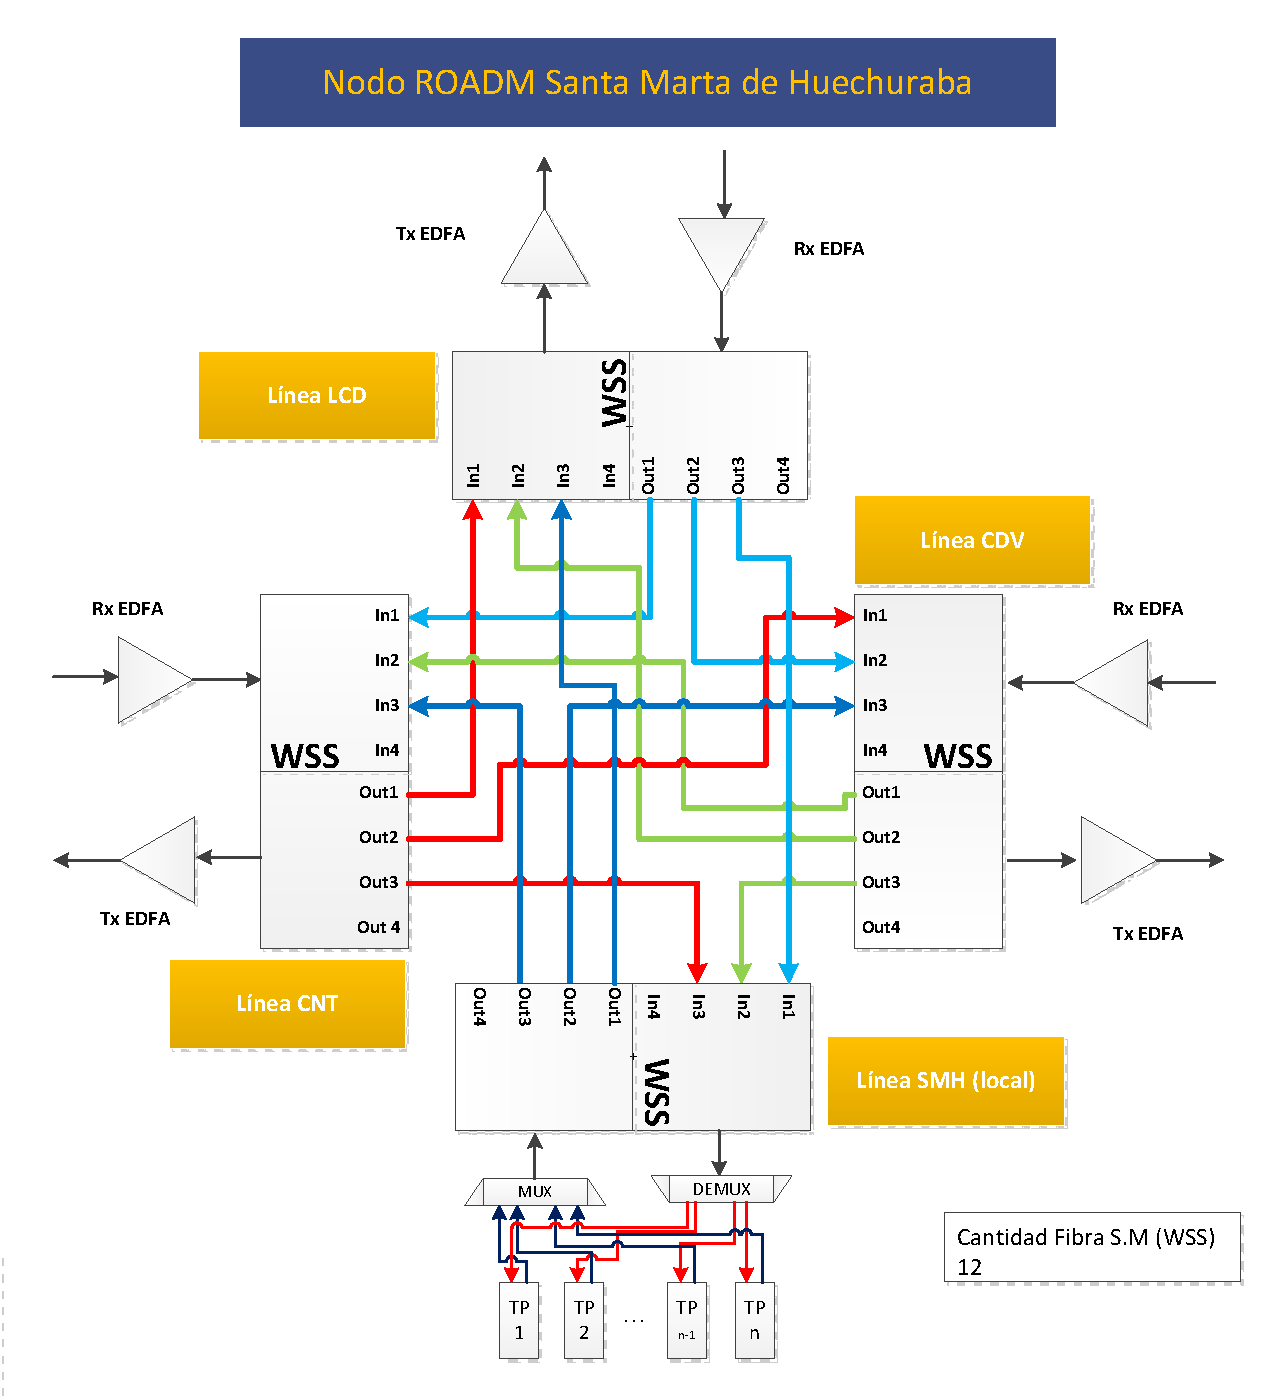
\includegraphics[width=17cm]{Imagenes/SMH.pdf}
  \caption{Diagrama de conexión de equipos para infrastructura ROADM en ``Santa Marta de Huechuraba''}
  \label{fig:drsmh}
\end{figure}

% Conjunto de documentacion tecnica de cada elemento usado en el proyecto
% 
\newpage
\section{Estimación del SLA}
\label{sec:SLA}

El acrónimo \emph{SLA} corresponde a las siglas de \emph{Service Level
Agreement} o de Acuerdo de Nivel de Servicio. Este documento corresponde 
a un contrato entre el proveedor y un cliente para respaldar legalmente 
que el servicio cumple ciertos estándares de calidad concretos, como 
disponibilidad (\emph{uptime}), tiempo medio entre fallas (\emph{MTBF}),
tiempo medio de reposición de servicio (\emph{MTTR}), etcétera.

El \emph{SLA} es, en este caso, algo que se debe determinar a partir de 
las características del diseño del proyecto. Esto se debe a que existe 
una cierta infraestructura que será aprovechada para cumplir los 
objetivos buscados.

Entre los diversos elementos que permite garantizar el \emph{SLA} de
una red destacan:
\begin{itemize}
\item Servicios prestados
\item Parámetros de QoS:
  \begin{itemize}
  \item Throughput
  \item Ancho de banda medio
  \item Latencia máxima
  \item Interrupciones máximas
  \item Probabilidad de indisponibilidad de red
  \end{itemize}
\item Tarifas y facturación
\end{itemize}

Una forma en que puede variar el \emph{SLA} y que está considerado
entre las restricciones del proyecto es la probabilidad de cortes de
los cables.

\subsection{Modelo Probabilístico de la red}

La red de fibra oscura actual se compone de 6 data centers ubicados 
en la ciudad de Santiago y sus alrededores. La red posee cables de 
fibra oscura G.652.D que permiten el uso de 96 fibras ópticas en cada 
uno. Este tipo de fibra presenta una tasa de cortes anual de $0.05 
[\frac{\text{cortes}/\text{año}}{\text{km}}]$ en zona metropolitana y 
$0.01 [\frac{\text{cortes}/\text{año}}{\text{km}}]$ en zona rural. 
Debido a esto, es se espera que cada cierto tiempo, el camino que 
utilizaba la red para conectar un par de data centers esté 
inhabilitado y se requieran rutas alternativas con el fin de mantener 
un estándar de calidad en disponibilidad de conexión en la red.

Se define la probabilidad de que una conexión física (cable de fibra 
óptica G.652.D) entre 2 \emph{datacenters} separados por una distancia 
$L$, se encuentre inhabilitada por cierto periodo de tiempo $\Delta T$, 
como la probabilidad acumulada en el tiempo de $\Delta T$ (en días) 
según la tasa de corte anual por Km $R$ (en $\frac{\text{cortes}/\text{año}}{\text{km}}$) \eqref{proba_corte_1}.

\begin{equation}
\label{proba_corte_1}
P(\text{corte físico en }\Delta T) = L R \Delta T /365
\end{equation}

Luego se puede extender el concepto de conexión física entre dos 
\emph{datacenters} incluyendo los nodos de paso. La probabilidad de 
corte en este caso se calcula como el máximo de la probabilidad de 
corte de cualquiera de las conexiones entre los nodos pertenecientes al 
camino \eqref{proba_corte_2}.

\begin{equation}
\label{proba_corte_2}
P(\text{corte físico en }\Delta T) = \max_{i \in \text{Conexiones del Camino}} {L_i R_i \frac{\Delta T}{ 365}}
\end{equation}

El valor de esta probabilidad se puede reducir al agregar vías 
alternativas para conectar los dos \emph{datacenters}. Considerando 
independientes los sucesos que implican un corte en el cable, la 
probabilidad de indisponibilidad para la conexión entre ambos 
\emph{datacenters} será el producto de las probabilidades corte de cada 
camino \eqref{proba_corte_3}.

\begin{equation}
\label{proba_corte_3}
P(\text{indisponibilidad entre data centers A y B en }\Delta T) =  \prod_{j \in \text{Caminos}}\left( \frac{\Delta T}{365}\right) \max_{i \in \text{Conex. del Camino}} {L_{i,j} R_{i,j} }
\end{equation}

Dado que la tasa de cortes depende del tipo de zona en el que está 
inserto el \emph{datacenter}, la tasa de corte $R$ depende del camino 
que toma la conexión. Este modelo pretende establecer una estimación de 
la probabilidad de indisponibilidad de la conexión de cada par de 
\emph{datacenters}. Se escogió el periodo $\Delta T$ como el tiempo que 
los técnicos demoran en hacer las reparaciones en el corte de manera tal 
que la red vuelva a su estado normal. Este período se estima en torno a 
los 2 días como máximo según datos de referencia.

\subsection{Algortimo de cálculo de Conexiones}
\label{sec:algoritmo_conex}

La idea detrás de este algoritmo consiste en determinar un número fijo 
de vías de conexión entre cada par de \emph{datacenters} para cumplir 
con el \emph{SLA}. En otras palabras, se busca poder aseverar que la 
probabilidad de falla en la conexión entre dos \emph{datacenters} es 
menor a $0.01 \%$ dada una ventana de tiempo de 2 días, luego de la cual
se asume que esta falla será reparada.

Para obtener una red que sea capaz de cumplir con estos requerimientos 
se requiere que la expresión de la ecuación \eqref{proba_corte_3} esté 
acotada por este porcentaje ($0.01\%$). 

De esta forma, el algoritmo a utilizar es el siguiente: para cada par 
de \emph{datacenters} se procede de forma iterativa buscando los caminos 
que representan una menor distancia utilizando el algoritmo de Dijkstra
para optimización de grafos. Luego se calcula la probabilidad de corte 
\eqref{proba_corte_3} actual y la compara con el valor umbral. Si el 
valor umbral sigue siendo inferior, se remueve el último camino propuesto 
y se agrega el siguiente camino óptimo. Este proceso se repite hasta que 
se obtenga la probabilidad deseada o se acaben los caminos factibles.

Los resultados obtenidos por el algoritmo se muestran en la figura
\ref{fig:caminos}

\begin{figure}[H]
  \centering
  %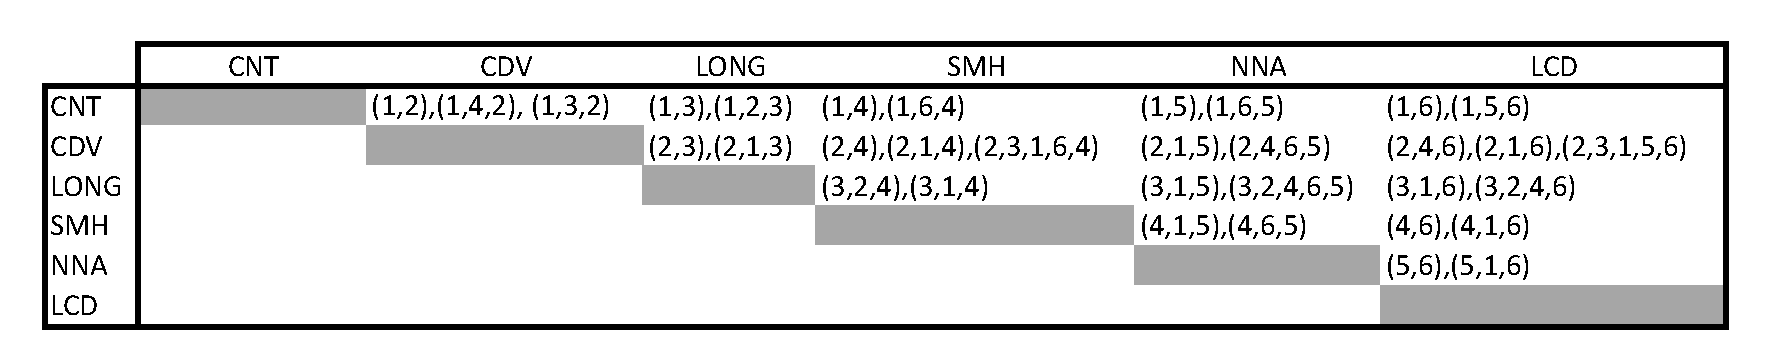
\includegraphics[width=13cm]{Imagenes/caminos}
  \caption{Caminos que pueden utilizar los datacenters para la comunicaciones, determinados según el algoritmo que fija la probabilidad de indisponibilidad.}
  \label{fig:caminos}
\end{figure}


\subsection{Efecto de la probabilidad de cortes de cable en el SLA}
\label{sec:cortes}

En una infraestructura de red oscura, un corte de cable entre dos data
centers significa que todas las conexiones entre esos data centers
quedan suspendidas hasta que los cables sean reparados físicamente
(introduciendo el valor \emph{MTTR}). Ello repercute directamente
en el \emph{SLA}, reduciendo el índice de interrupciones máximas.

Afortunadamente, el desarrollo actual permite acceder a la tecnología 
de conmutación dinámica de red ópticas de forma mucho más fácil
que hace algunos años. Acceder hoy a arquitecturas basadas en
\emph{WSON}, \emph{ROADM} y \emph{WSS} no aumenta significativamente el 
\emph{CAPEX}, \emph{OPEX} o la complejidad del proyecto, pero sí afecta 
sustancialmente al \emph{SLA}, introduciendo mejoras al índice de 
interrupciones máximas al reducir considerablemente el \emph{MTBF}.

Por otro lado, se pueden utilizar estimaciones de probabilidades de corte ...

\subsection{Garantías en cuanto al ancho de banda y \emph{throughput}
  de la red óptica}
\label{sec:anchodebanda}

Entre las especificaciones del proyecto, se pide un cierto número y
tipo de servicios para comunicaciones entre los \emph{datacenters}. Los
equipos instalados tras el diseño propuesto en este informe tienen la
obligación de dejar instalada la capacidad pedida en cada caso.

Las capacidades pedidas por \emph{datacenter} y por protocolo de
transmisión se muestran en las tablas \ref{tab:10ge} y \ref{tab:FC4G}.

\begin{table}[H]
  \centering
  \begin{tabular}{| l | c | c | c | c | c | c |}
    \hline
    \textbf{10GE} & \textbf{CNT} & \textbf{CDV} & \textbf{LONG} & \textbf{SMH} & \textbf{NNA} & \textbf{LCD} \\
    \hline
    \textbf{CNT}  & - & 20 & 10 & 4 & 4 & 6 \\
    \hline
    \textbf{CAD}  &   & - & 10 & 4 & 4 & 4 \\
    \hline
    \textbf{LONG} &   &   & - & 6 & 4 & 4 \\
    \hline
    \textbf{SMH}  &   &   &   & - & 4 & 4 \\
    \hline
    \textbf{NNA}  &   &   &   &   & - & 4 \\
    \hline
    \textbf{LCD}  &   &   &   &   &   & - \\
    \hline
  \end{tabular}
  \caption{Número de servicios entre data centers para protocolo 10GE}
  \label{tab:10ge}
\end{table}

 \begin{table}[H]
   \centering
   \begin{tabular}{| l | c | c | c | c | c | c |}
     \hline
     \textbf{FC 4G} & \textbf{CNT} & \textbf{CDV} & \textbf{LONG} & \textbf{SMH} & \textbf{NNA} & \textbf{LCD} \\
     \hline
     \textbf{CNT}  & - & 30 & 20 & 4 & 4 & 6 \\
     \hline
     \textbf{CAD}  &   & - & 20 & 4 & 4 & 4 \\
     \hline
     \textbf{LONG} &   &   & - & 6 & 4 & 4 \\
     \hline
     \textbf{SMH}  &   &   &   & - & 4 & 4 \\
     \hline
     \textbf{NNA}  &   &   &   &   & - & 4 \\
     \hline
     \textbf{LCD}  &   &   &   &   &   & - \\
     \hline
   \end{tabular}
   \caption{Número de servicios entre data centers para protocolo Fiber Channel 4G}
   \label{tab:FC4G}
 \end{table}

% Garantías que da el proovedor al consumidor.
\newpage
\section{Evaluaci\'on }\label{sec:evaluacion}

\subsection{CAPEX}

Para este punto de la planificación del proyecto, es importante
visualizar todos los componentes del proyecto y la cantidad de horas
hombre en ingeniería y en instalación de equipos que se destinarán. Es
importante visualizar, especialmente, los componentes con los que no
se cuenta inicialmente, siendo necesaria la 

La instalación inicial de fibra tipo G.652.D permite ahorrarse este componente de la 

% Monto total de las inversiones requeridas para la ejecución completa de un proyecto. Se 
% incluyen por lo tanto los siguientes ítems: 

% Equipos de telecomunicaciones, generalmente importados 
% Equipos de poder y clima (rectificadores, bancos de baterías, equipos de aire 
% acondicionado) 
% Materiales de instalación 
% Stock de unidades de repuesto 
% Licencias de software requeridas para la gestión de los equipos 
% Pre-ingeniería 
% Ingeniería de detalle 
% Instalación y Puesta en marcha 
% Administración del proyecto 
% Capacitación 
 
% Los primeros cuatro elementos se explican por sí solos. Algunos comentarios sobre los 
% restantes: 
 
% La pre-ingeniería considera las actividades previas a la ejecución del proyecto mismo como 
% visitas a terreno para definir ubicación física de los equipos, determinación de la existencia de 
% recursos de poder (alimentación continua -48 VDC) disponibles para los equipos, asignación de 
% automáticos, posiciones de las fibras ópticas en los ODF, etc. 
 
% En algunos casos, con proyectos que incluyan enlaces de microondas, la pre-ingeniería es 
% más compleja, ya que requiere definición de ubicación de estaciones de radio, pruebas de 
% despeje radioeléctrico, predicción de comportamiento de los radioenlaces, etc. 


% CAPEX Y OPEX.
\newpage
\section{Conclusiones}\label{sec:conclusiones}

Las redes ópticas pueden ser diseñadas de manera flexible usando
tecnologías que permiten multiplexar y manejar una gran cantidad de
señales de forma confiable y eficiente en una sola fibra óptica. Esto
se puede hacer de forma escalonada, instalando equipos que conformen
una red óptica \emph{DWDM}.

Los costos de estas implementaciones no son nada fuera de lo común y
día a día disminuyen más los precios. Los sistemas de fibra oscura han
perdido terreno en el mercado por su baja escalabilidad y poca
flexibilidad.

Se han agregado funcionalidades al tendido inicial de fibra oscura que
se traducen en una mejor calidad de servicio, al idear una forma de
diseñar la red óptica a partir de un requerimiento que define al
\emph{SLA}.

Se ha evaluado cada uno de los dispositivos que conforma a la red de
manera descentralizada, y se ha obtenido el CAPEX y OPEX del primer
año de una red de estas características.

%% Adding references page
\newpage
%\section{References}

%\bibliographystyle{ieeetr}
%\bibliographystyle{acm}
%\bibliographystyle{apalike}
%\nocite{*}
	
%\bibliography{Referencias/referencias}

\begin{thebibliography}{9}

% JF: Creo que conviene mas citar el documento oficial G.652
\bibitem{G652D}
  International Telecommunication Union,
  \emph{Transmission Media and Optical Systems Characteristics - Optical Fibre Cables},
  Series G: Transmission Systems and Media, Digital Systems and Networks,
  2009.

\bibitem{datasheetfibra}
  TELNET Redes Inteligentes S.A.,
  \emph{Monomode Optical Fiber G.652.D}.
  \url{http://www.telnet-ri.es/fileadmin/user_upload/hojas_producto_EN/CABLES_FO/Fibra_SM_G.652.D_EN_V1.0.pdf}
  
\bibitem{bandasdwdm}
  Camilo Garc\'ia Morales,
  \emph{Sistemas de Transmisi\'on - DWDM y CWDM},
  Instituci\'on Universitaria de Envigado,
  2012.
  \url{http://sx-de-tx.wikispaces.com/DWDM+y+CWDM}

\end{thebibliography}
%% Appendix
%\newpage
%\input{Secciones/anexo}




\end{document}
